% ================ CHAPTER 4 — DESIGN, IMPLEMENTATION, AND EVALUATION ================
This chapter presents the architecture, detailed design, implementation, testing,
and deployment of the system.

\section{Architecture Design}

\subsection{Software Architecture Selection}
% GUIDE (1-3 pages): choose & briefly explain the architecture: a 3-tier, layered
% client-server design — React SPA (presentation) / Spring Boot REST (controller-
% service-repository) / PostgreSQL (data). Then map the layers to this system.
\thesisfig{architecture}{Overall system architecture}{fig:architecture}
The system adopts a three-tier client-server architecture, as shown in
Figure~\ref{fig:architecture}. The presentation tier is a React single-page
application that runs in the user's browser. It is responsible for rendering
forms, tables, dashboards, navigation, and status feedback. The application tier
is a Spring Boot REST backend. It exposes API endpoints, authenticates requests,
checks authorization, executes business rules, and coordinates transactions. The
data tier is PostgreSQL, which stores master data, business documents,
inventory, lots, invoices, delivery records, and user-role information.

This architecture was selected because the system contains many business
workflows that must be consistent across modules. If the frontend directly
handled inventory rules, each screen would need to repeat the same validation
logic. Instead, all core rules are centralized in backend services. For example,
sales order approval checks available inventory and reserves stock; goods
receipt confirmation updates purchase order progress and creates lots; goods
issue confirmation deducts stock by FEFO and creates an invoice. The frontend
only calls the relevant API and displays the result.

The architecture also supports maintainability. Each tier can evolve with a
clear boundary: the frontend focuses on user experience, the backend focuses on
business logic, and the database focuses on persistence and integrity. This is
appropriate for the thesis because the project must demonstrate both a usable
application and non-trivial business rules without mixing responsibilities.

\subsection{Overall Design}
% GUIDE: UML package diagram organised by layers; explain each package's responsibility
% and the dependency rules (upper depends on lower only).
\thesisfig{package_diagram}{Package diagram (layered backend)}{fig:packages}
Figure~\ref{fig:packages} presents the main backend packages. The
\texttt{controller} package contains REST controllers for authentication,
master data, purchase orders, goods receipts, sales orders, goods issues,
delivery, inventory, invoices, accounting, payments, dashboard, and user
management. Controllers
convert HTTP requests into DTOs and delegate processing to services. The
\texttt{dto} package contains request and response objects used between the
frontend and backend, preventing entity classes from being exposed directly.

The \texttt{service} package defines business interfaces and the
\texttt{service.impl} package implements them. This is the main location of
workflow logic such as purchase approval, sales approval, inventory reservation,
FEFO goods issue, failed-delivery recovery, and dashboard aggregation. The
\texttt{repository} package contains Spring Data repositories and custom queries
for persistence. The \texttt{model} package contains JPA entities, while
\texttt{model.enums} contains lifecycle states such as purchase order status,
sales order status, goods receipt status, goods issue status, invoice status,
payment status, and role type.

Supporting packages are separated from domain packages. The \texttt{security}
package implements JWT token generation, authentication filtering, custom user
details, and role annotations. The \texttt{config} package defines security,
CORS, and API documentation configuration. The \texttt{exception} package
provides domain exceptions and a global exception handler. The
\texttt{scheduler} package contains scheduled background jobs; currently it
holds the overdue-invoice job, which runs daily and marks unpaid invoices past
their due date as overdue. The dependency
direction follows the layered rule: controllers depend on services and DTOs,
services depend on repositories and models, and repositories depend on models.
Lower layers do not call upper layers.

\subsection{Detailed Package Design}
% GUIDE: class diagrams (names + relationships only) per related package group.
\thesisfig{class_inbound}{Class diagram — inbound (purchasing) flow}{fig:class-in}
\thesisfig{class_outbound}{Class diagram — outbound (sales) flow}{fig:class-out}
\thesisfig{class_delivery}{Class diagram — delivery flow}{fig:class-dlv}
The inbound package group in Figure~\ref{fig:class-in} models the
procure-to-stock process. A supplier is associated with purchase orders, and
each purchase order contains multiple purchase order items. A goods receipt is
created from an approved or partially received purchase order and contains goods
receipt items. When a goods receipt is confirmed, accepted quantities update the
purchase order items, aggregate inventory, inventory transactions, and lot
records. This design keeps the original purchase document, the warehouse
receipt, and the resulting inventory movement traceable.

The outbound package group in Figure~\ref{fig:class-out} models the
order-to-cash process. A customer places a sales order with sales order items.
After approval, stock is reserved in the selected warehouse. A goods issue is
then created from the approved sales order and contains goods issue items. When
the goods issue is confirmed, stock is deducted, lots are consumed according to
FEFO, delivered quantities are updated, and a sales invoice is generated. This
group is the core of the inventory-reservation and FEFO contribution described
in Chapter~\ref{chapter:Contribution}.

The delivery package group in Figure~\ref{fig:class-dlv} models planning and
execution after goods issue. Delivery plans group delivery orders and assign
shipper users through delivery plan shipper records. Delivery trip routes and
route items represent executable trips. Shippers update delivery status, while
delivery administrators manage planning and assignment. This separation allows
delivery execution to reference sales and goods issue documents without changing
their core structure.

\section{Detailed Design}

\subsection{User Interface Design}
% GUIDE (2-3 pages): state display standards (resolution, colour scheme, button/
% control conventions, feedback placement). Show UI MOCKUPS (prototypes, e.g. Figma/
% draw.io), NOT production screenshots (those go in 4.3.3).
The user interface is designed as an operational dashboard rather than a
marketing website. The main layout uses a left navigation menu for modules and a
content area for lists, forms, detail pages, and dashboards. Tables are used for
high-volume objects such as purchase orders, sales orders, inventory records,
goods receipts, goods issues, invoices, customers, suppliers, products, and
warehouses. Forms are grouped by business meaning: header information appears at
the top, line items are edited in a table-like section, and action buttons are
placed near the document status.

The interface follows several standards. First, each business document displays
its code, status, partner, date, warehouse, monetary values, and line items in a
consistent order. Second, status is shown with color-coded tags so that users can
quickly distinguish draft, approved, confirmed, cancelled, partially delivered,
and completed records. Third, destructive or irreversible actions such as
confirmation, cancellation, and deletion require confirmation dialogs. Fourth,
validation errors are displayed close to the relevant form field, while
operation-level errors are displayed as notifications.

Because the system has been fully implemented and deployed, these design standards
are not illustrated through separate prototype mockups but through the realized
screens of the running application, which are presented and explained in
Section~\ref{sec:main-functions}. Presenting the delivered interface rather than a
prototype keeps the design description consistent with the system that was actually
built: the left-navigation layout, the consistent document header, the color-coded
status tags, and the confirmation dialogs described above can be observed directly
in those screenshots, for example the document layout and status tag in
Figure~\ref{fig:ui-po} and the color-coded inventory status in
Figure~\ref{fig:ui-inventory}.

\subsection{Layer Design}
% GUIDE (3-4 pages): detailed design (attributes + methods) of 2-4 key classes,
% plus sequence diagrams for 2-3 important use cases.
\thesisfig{class_detail_key}{Detailed design of key classes}{fig:class-detail}
\thesisfig{seq_so_gi_fefo}{Sequence — confirm Goods Issue with FEFO allocation}{fig:seq-fefo}
\thesisfig{seq_po_gr}{Sequence — approve PO and confirm Goods Receipt}{fig:seq-pogr}
\thesisfig{seq_delivery_trip}{Sequence — assign and execute delivery trip}{fig:seq-trip}
Figure~\ref{fig:class-detail} focuses on the key classes that carry the most
important business rules. \texttt{Inventory} stores aggregate stock quantities,
including on-hand, reserved, and available quantities. \texttt{InventoryLot}
stores batch-level quantity and expiry information. \texttt{SalesOrder} and
\texttt{SalesOrderItem} represent customer demand and delivered progress.
\texttt{GoodsIssue} and \texttt{GoodsIssueItem} represent the warehouse outbound
document and record the batch information used during FEFO allocation.
\texttt{GoodsReceipt} and \texttt{GoodsReceiptItem} represent inbound warehouse
confirmation and are the source for lot creation.

The sequence in Figure~\ref{fig:seq-fefo} starts when a warehouse staff member
confirms a goods issue. The controller calls the goods issue service, which
loads the goods issue with its items, validates the document status, acquires a
pessimistic write lock on the aggregate inventory row of each product,
checks physical stock, retrieves available lots in FEFO order, deducts lot
quantities, decreases aggregate inventory, releases reserved stock, updates
delivered quantities, creates a sales invoice, and updates the sales order
delivery status. The lock taken before any lot is read serializes concurrent
confirmations of the same product, as analysed in
Chapter~\ref{chapter:Contribution}. The sequence shows why this operation must be
transactional: every change belongs to one business event.

The sequence in Figure~\ref{fig:seq-pogr} shows the inbound flow. A purchase
order is approved first. A warehouse staff member then creates and confirms a
goods receipt. Confirmation validates the remaining ordered quantity, increases
aggregate inventory, creates an inventory transaction, creates inventory lots
from accepted quantities, and updates the purchase order receiving status. The
sequence in Figure~\ref{fig:seq-trip} shows delivery assignment and execution:
delivery administrators build a plan and assign shippers, while shippers update
trip status. Failed delivery triggers the recovery mechanism described in
Chapter~\ref{chapter:Contribution}.

\subsection{Database Design}
% GUIDE (2-4 pages): E-R diagram + explanation; then the physical schema (PostgreSQL).
\thesisfig{er_diagram}{Entity-Relationship diagram}{fig:er}
The database design in Figure~\ref{fig:er} follows the business document
structure of a distributor. Master data includes products, warehouses,
suppliers, customers, delivery addresses, users, and roles. Transactional data
is organized around document headers and document lines. Purchase orders have
purchase order items; goods receipts have goods receipt items and refer back to
purchase orders; sales orders have sales order items; goods issues have goods
issue items and refer back to sales orders; invoices have invoice items and
refer to goods issues where applicable.

Inventory is represented at two levels. The aggregate \texttt{inventory} table
stores stock by product and warehouse, including on-hand, reserved, available,
reorder level, and average cost. The \texttt{inventory\_lot} table stores lot
number, expiry date, received quantity, remaining quantity, unit cost, product,
warehouse, and source goods receipt item. This two-level model allows the system
to answer both operational questions, such as available stock by warehouse, and
traceability questions, such as which lot remains close to expiry.

The delivery model contains delivery plans, delivery orders, delivery plan
orders, delivery plan shippers, delivery trip routes, and delivery trip route
items. These tables separate planning from execution and allow a shipper to be
assigned only to specific trips. Foreign keys preserve the relationship between
delivery records and the sales/goods issue documents they execute. Status fields
are implemented as enums in the application and persisted as database values,
which keeps lifecycle transitions explicit in the service layer.

\section{Application Building}

\subsection{Libraries and Tools}
% GUIDE: list every language/library/tool WITH VERSION. (Pre-filled from pom.xml +
% package.json — verify versions against your project.)
Table~\ref{tab:tools} lists the languages, frameworks, libraries, and tools used
to build the system, together with their versions as declared in the backend
\texttt{pom.xml} and the frontend \texttt{package.json}.
\begin{table}[H]\centering
\caption{Libraries, frameworks and tools used}
\label{tab:tools}
\begin{tabular}{|l|l|l|}
\hline
\textbf{Purpose} & \textbf{Tool / Library} & \textbf{Version} \\ \hline
Backend language        & Java                    & 17 \\ \hline
Backend framework       & Spring Boot             & 3.1.4 \\ \hline
ORM / data access       & Spring Data JPA (Hibernate) & (Boot 3.1.4) \\ \hline
Security / tokens       & Spring Security, JJWT   & 0.12.3 \\ \hline
DB migration            & SQL migration scripts   & V1--V10 \\ \hline
API documentation       & SpringDoc OpenAPI       & 2.1.0 \\ \hline
Boilerplate reduction   & Lombok                  & (Boot-managed) \\ \hline
Build tool (backend)    & Maven                   & 3.x \\ \hline
Database                & PostgreSQL              & 14+ \\ \hline
Frontend library        & React                   & 18.2.0 \\ \hline
Frontend build tool     & Vite                    & 5.0.0 \\ \hline
UI components           & Ant Design (antd)       & 5.10.0 \\ \hline
HTTP client             & Axios                   & 1.4.0 \\ \hline
Routing                 & React Router DOM        & 6.11.1 \\ \hline
Charts                  & Recharts                & 3.8.1 \\ \hline
Date/time               & Day.js                  & 1.11.10 \\ \hline
IDE                     & IntelliJ IDEA / VS Code & -- \\ \hline
\end{tabular}
\end{table}

\subsection{Achievement}
% GUIDE: describe the delivered product and report statistics (LOC, #classes,
% #packages, source size). Compute with: cloc backend/src frontend/src
\begin{table}[H]\centering
\caption{Source-code statistics}
\label{tab:loc}
\begin{tabular}{|l|r|}
\hline
\textbf{Metric} & \textbf{Value} \\ \hline
Lines of code (backend, Java) & 11,821 \\ \hline
Lines of code (frontend, JS/JSX) & 10,575 \\ \hline
Number of Java classes & 176 \\ \hline
Number of backend packages & 12 \\ \hline
Database migration scripts & V1--V10 \\ \hline
\end{tabular}
\end{table}
The delivered prototype contains the core modules required by the thesis scope:
purchasing, goods receipt, inventory and lot management, sales order processing,
goods issue, sales invoice, accounting and customer payment, delivery planning,
shipper trip execution, dashboard reporting, authentication, and user-role
management. Table~\ref{tab:loc} summarises the source-code statistics. The
backend source code has 11,821 lines of Java in 176 classes under
\texttt{backend/src/main/java}, organised into 12 packages. The frontend source
code has 10,575 lines of JavaScript/JSX under \texttt{frontend/src}. These values
were measured with the \texttt{cloc} tool and exclude blank and comment lines.

\subsection{Illustration of Main Functions}
\label{sec:main-functions}
This section illustrates the principal functions of the deployed system through
screenshots captured from the running application. The figures are ordered to
follow one complete distribution cycle, from authentication through inbound
logistics, outbound fulfilment with lot allocation, delivery, and financial
settlement, so that the behaviour of the design presented in the previous
sections can be traced in practice.

\begin{figure}[H]\centering
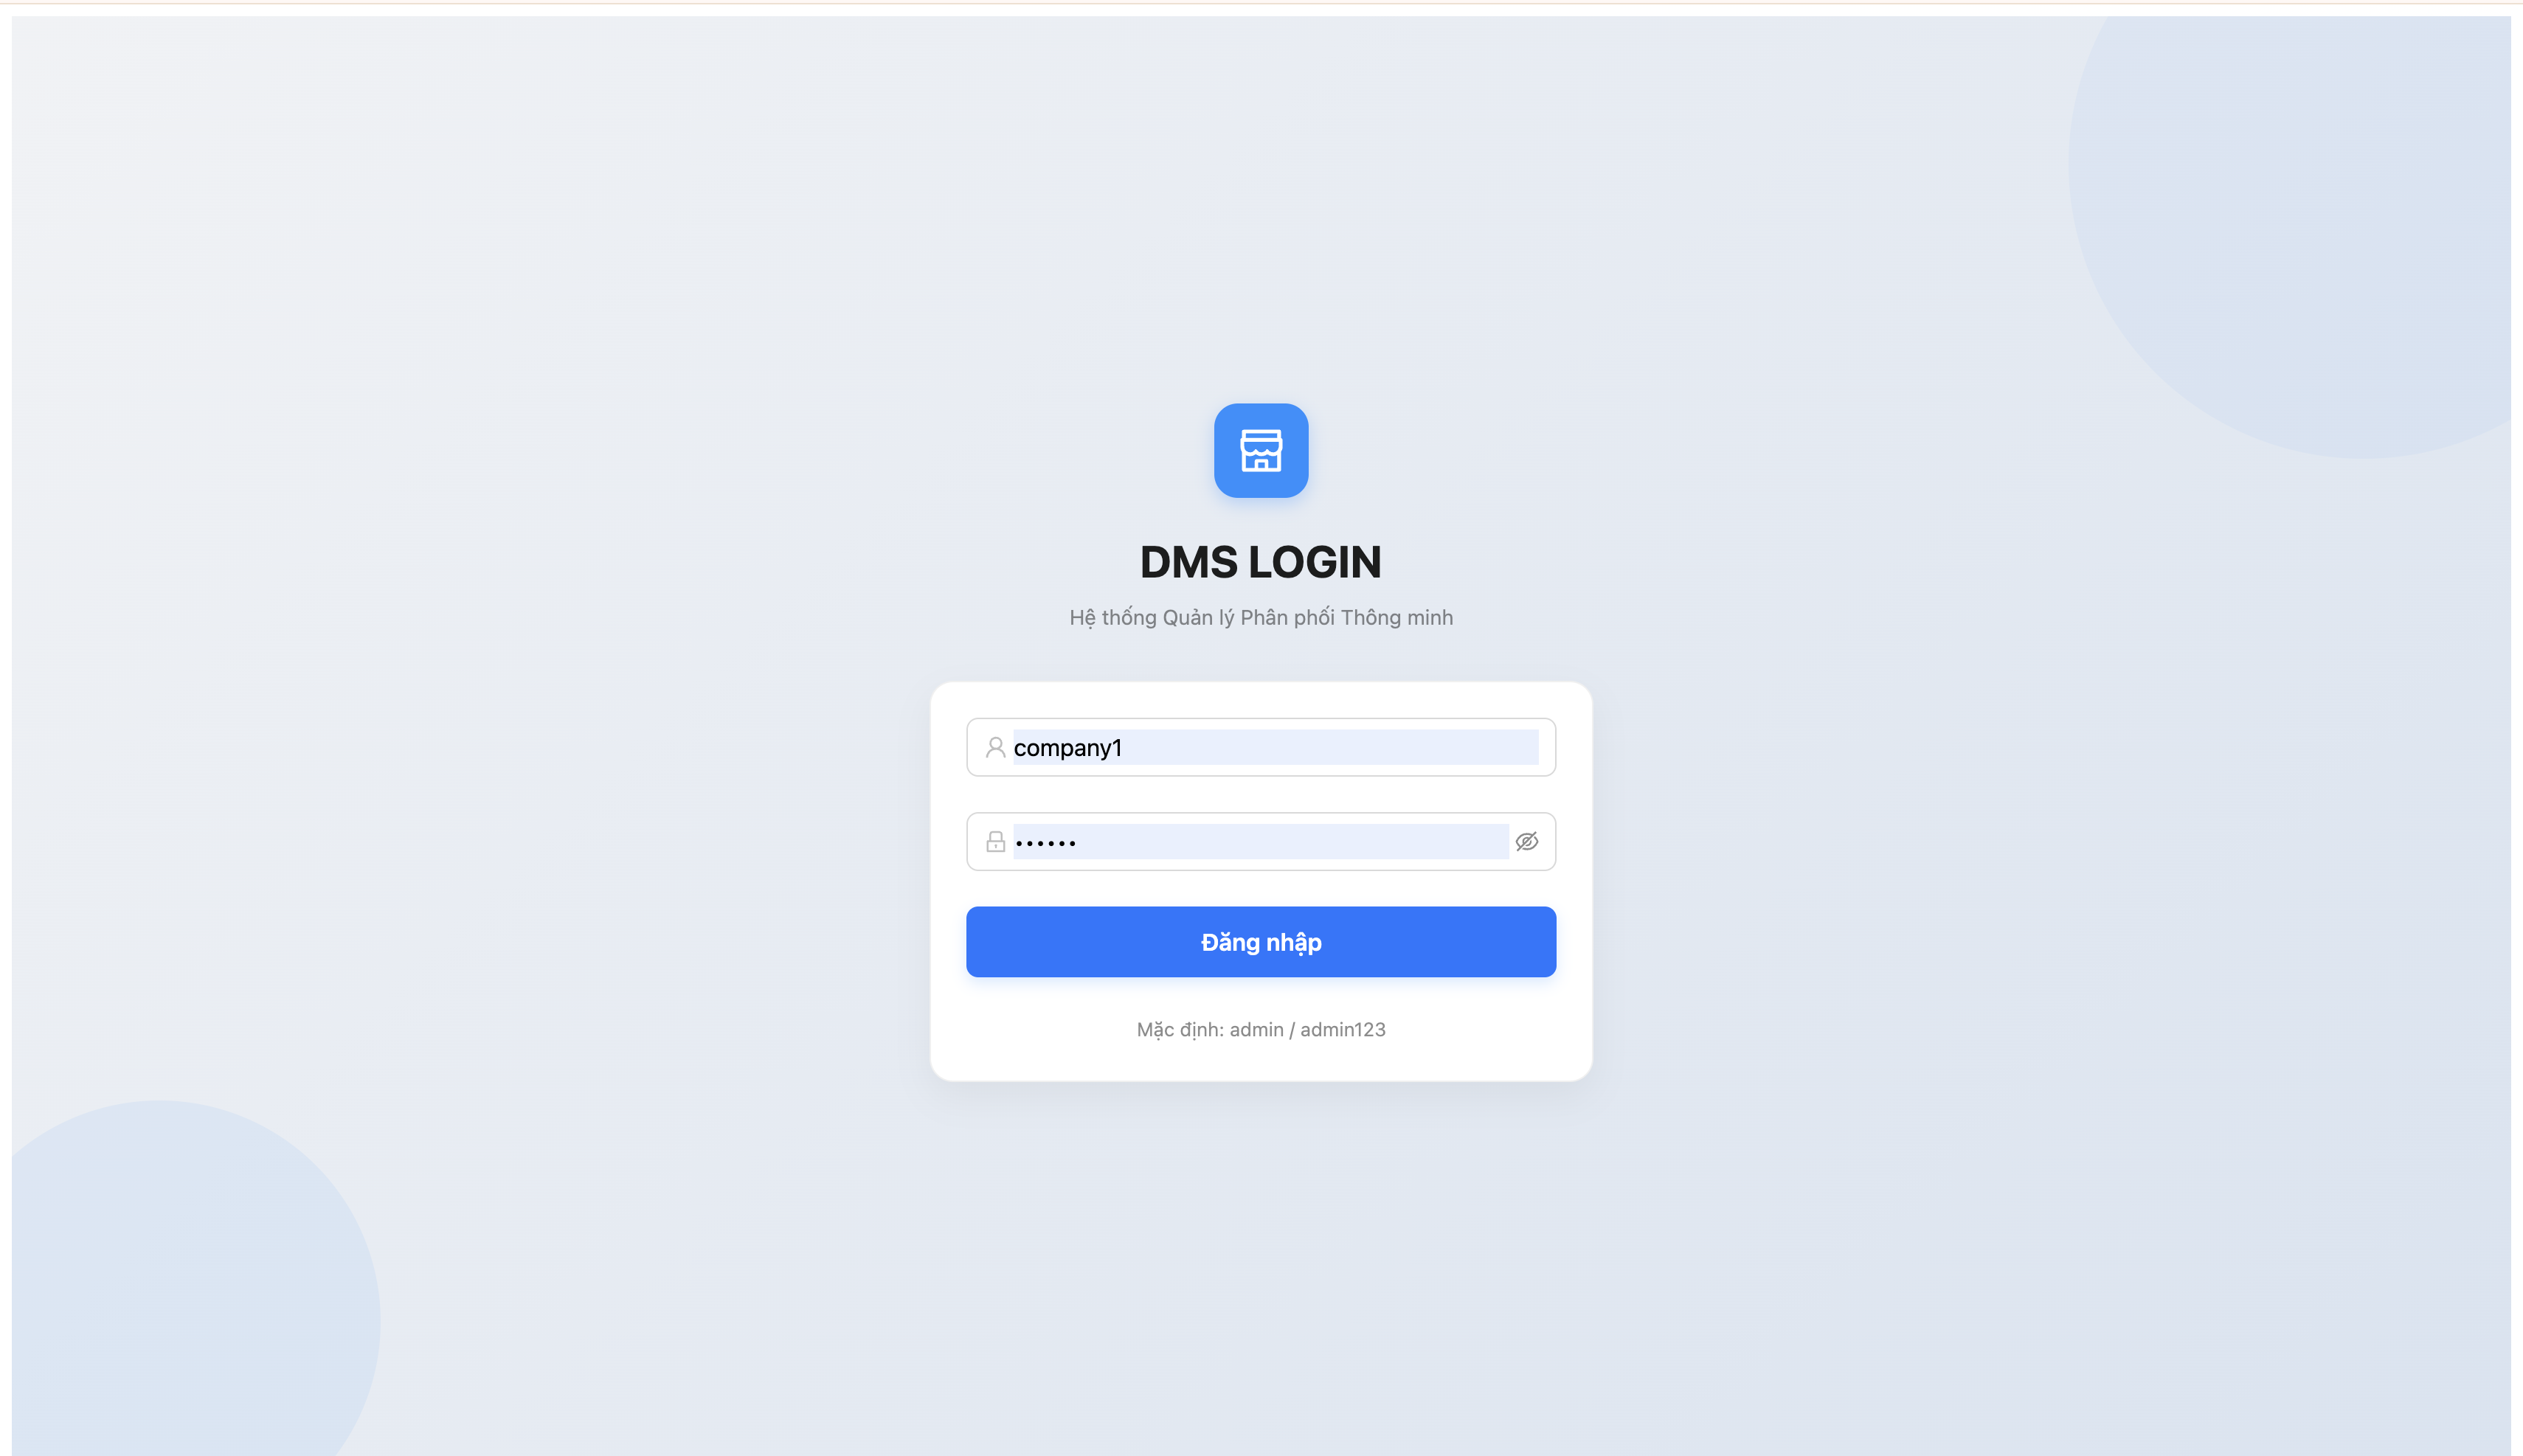
\includegraphics[width=0.62\linewidth]{Figure/screenshots/01-login.png}
\caption{Authentication screen}\label{fig:ui-login}
\end{figure}

Figure~\ref{fig:ui-login} shows the single sign-in screen through which every
user enters the system. Credentials submitted here are verified by the backend,
which returns a signed JSON Web Token that the browser then attaches to every
subsequent request; the routing and authorisation consequences of this token are
discussed in Section~\ref{sec:deployment}. Because all functional pages are
guarded, this screen is the only one reachable without a valid session.

\begin{figure}[H]\centering
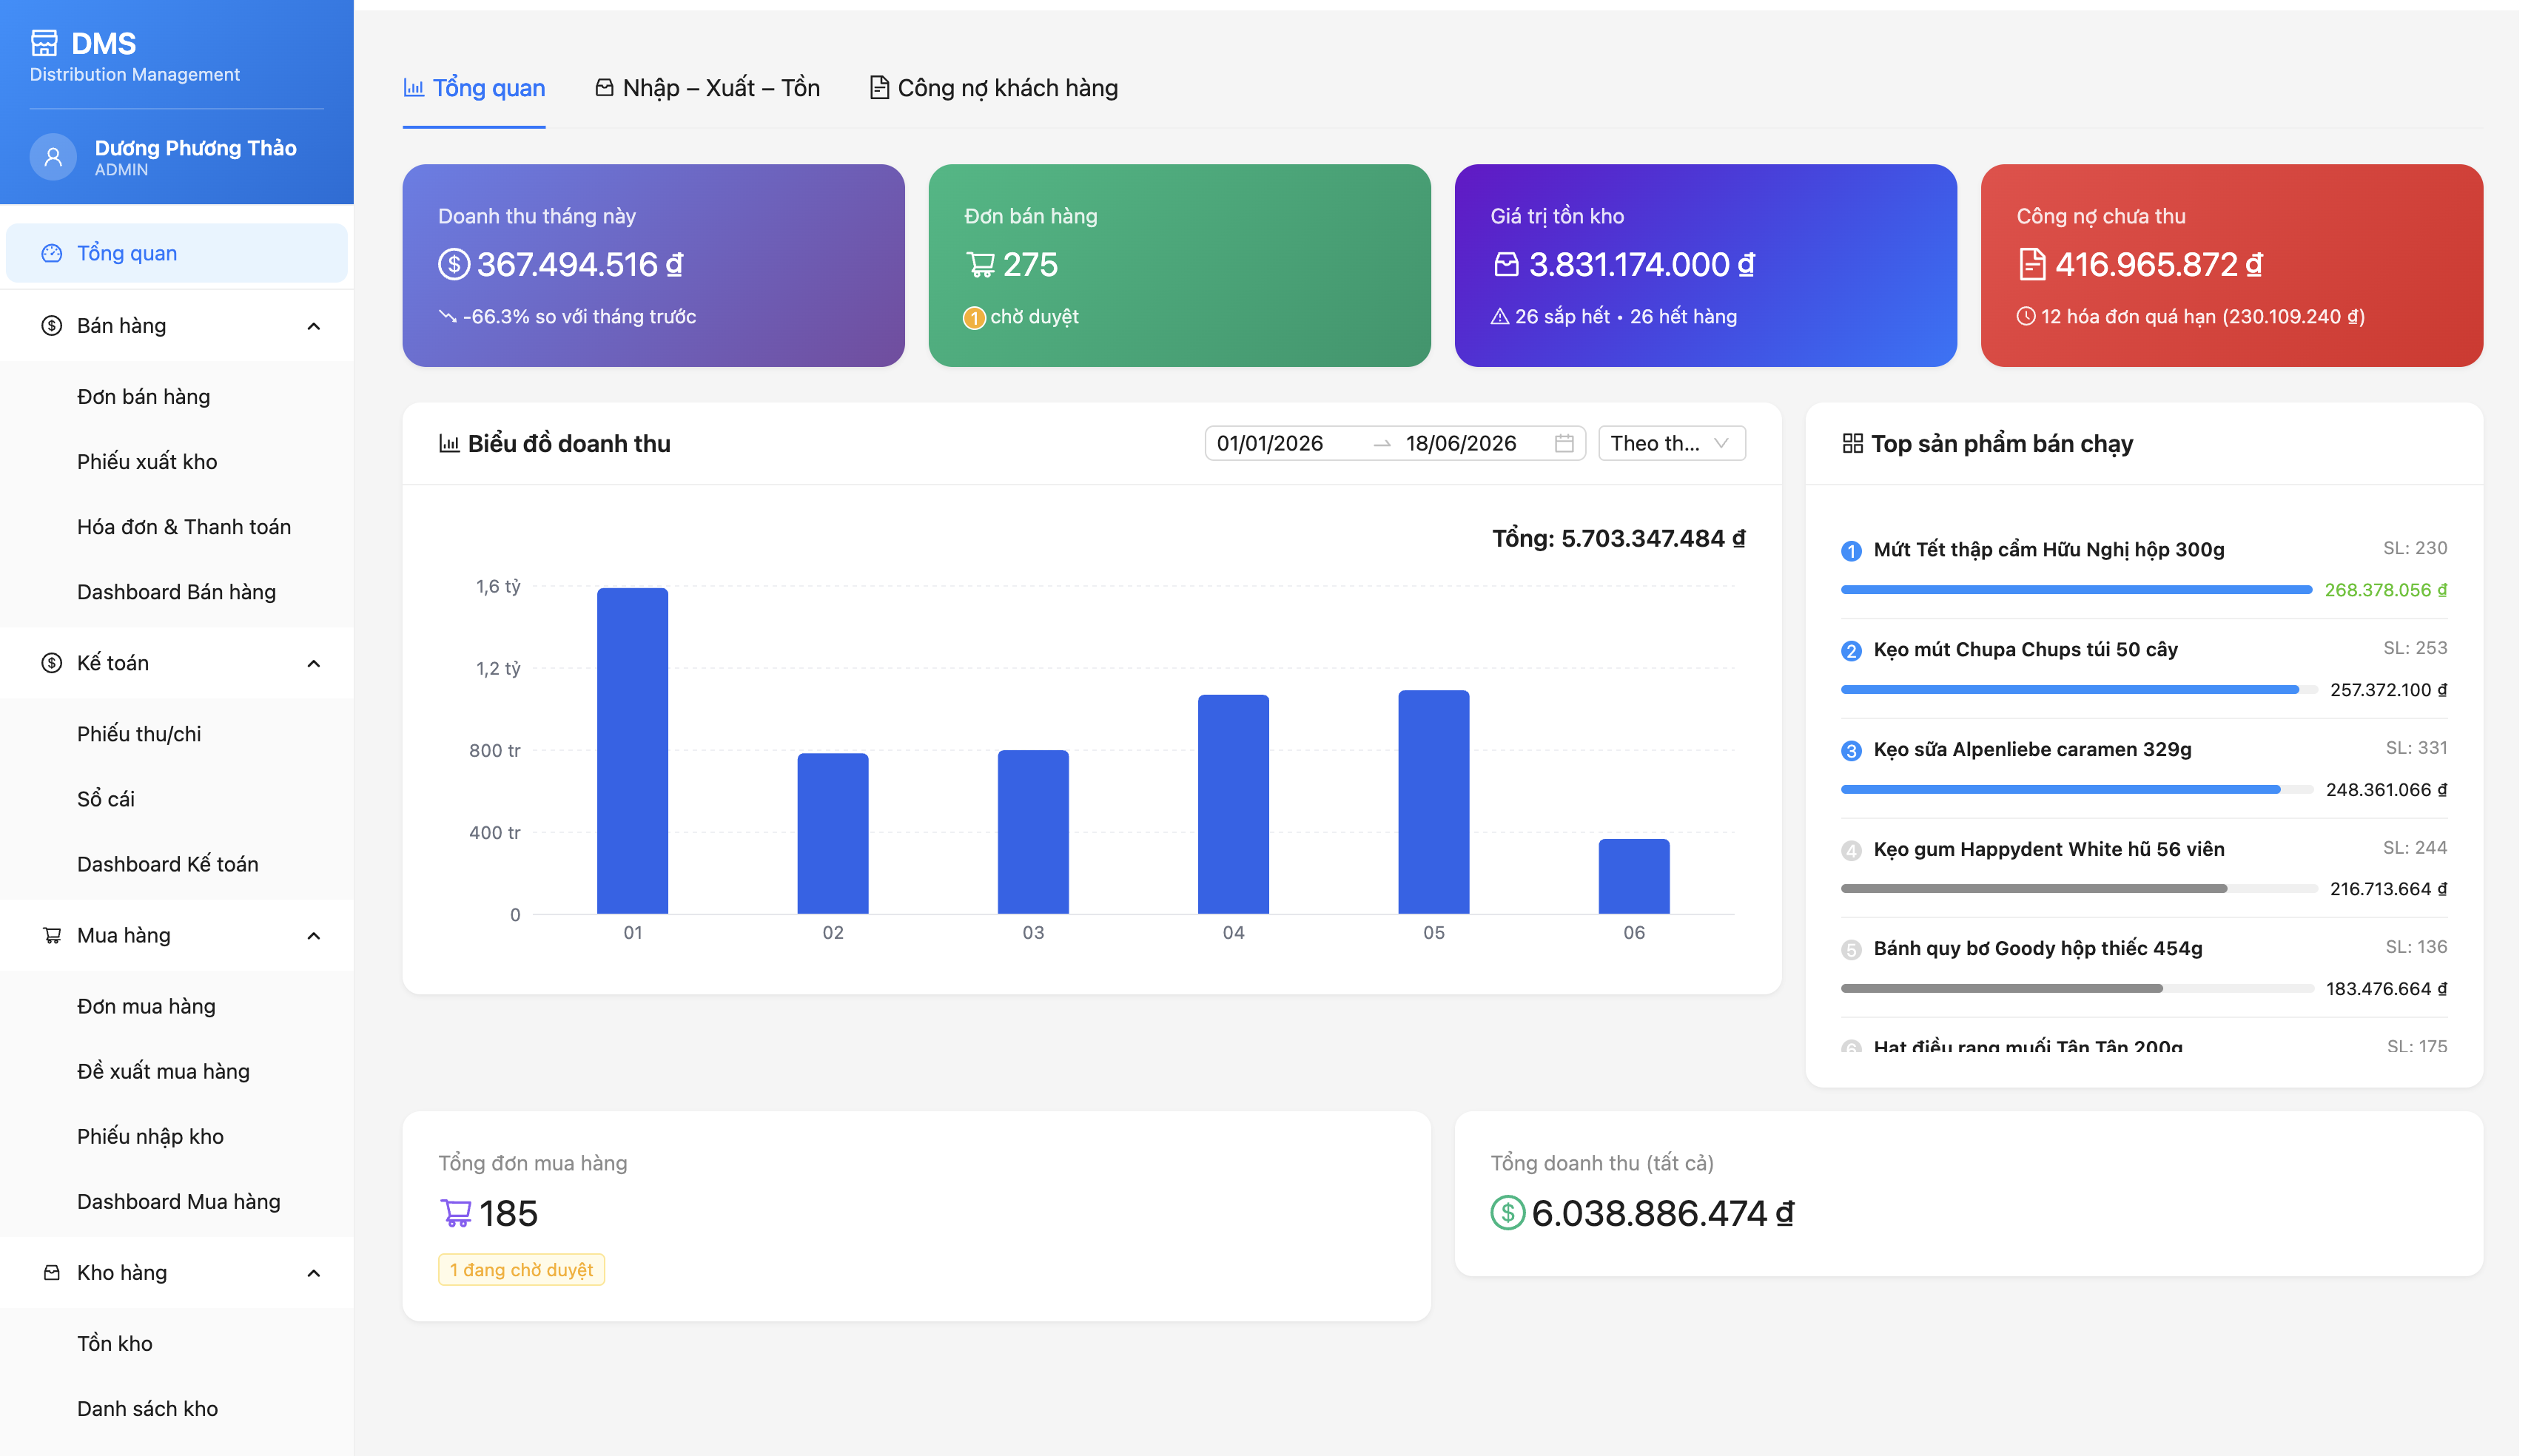
\includegraphics[width=0.95\linewidth]{Figure/screenshots/02-dashboard.png}
\caption{Management dashboard with aggregate indicators}\label{fig:ui-dashboard}
\end{figure}

Figure~\ref{fig:ui-dashboard} presents the management dashboard. Four
key-performance-indicator cards summarise (i) current-month revenue, (ii) the
number of sales orders, (iii) the total monetary value of stock on hand, and
(iv) outstanding accounts receivable, while a revenue chart and a
best-selling-product ranking give a quick operational overview. These figures are
aggregated on the server from the transactional tables rather than computed in
the browser, so the dashboard reflects the same data that drives the rest of the
application.

\begin{figure}[H]\centering
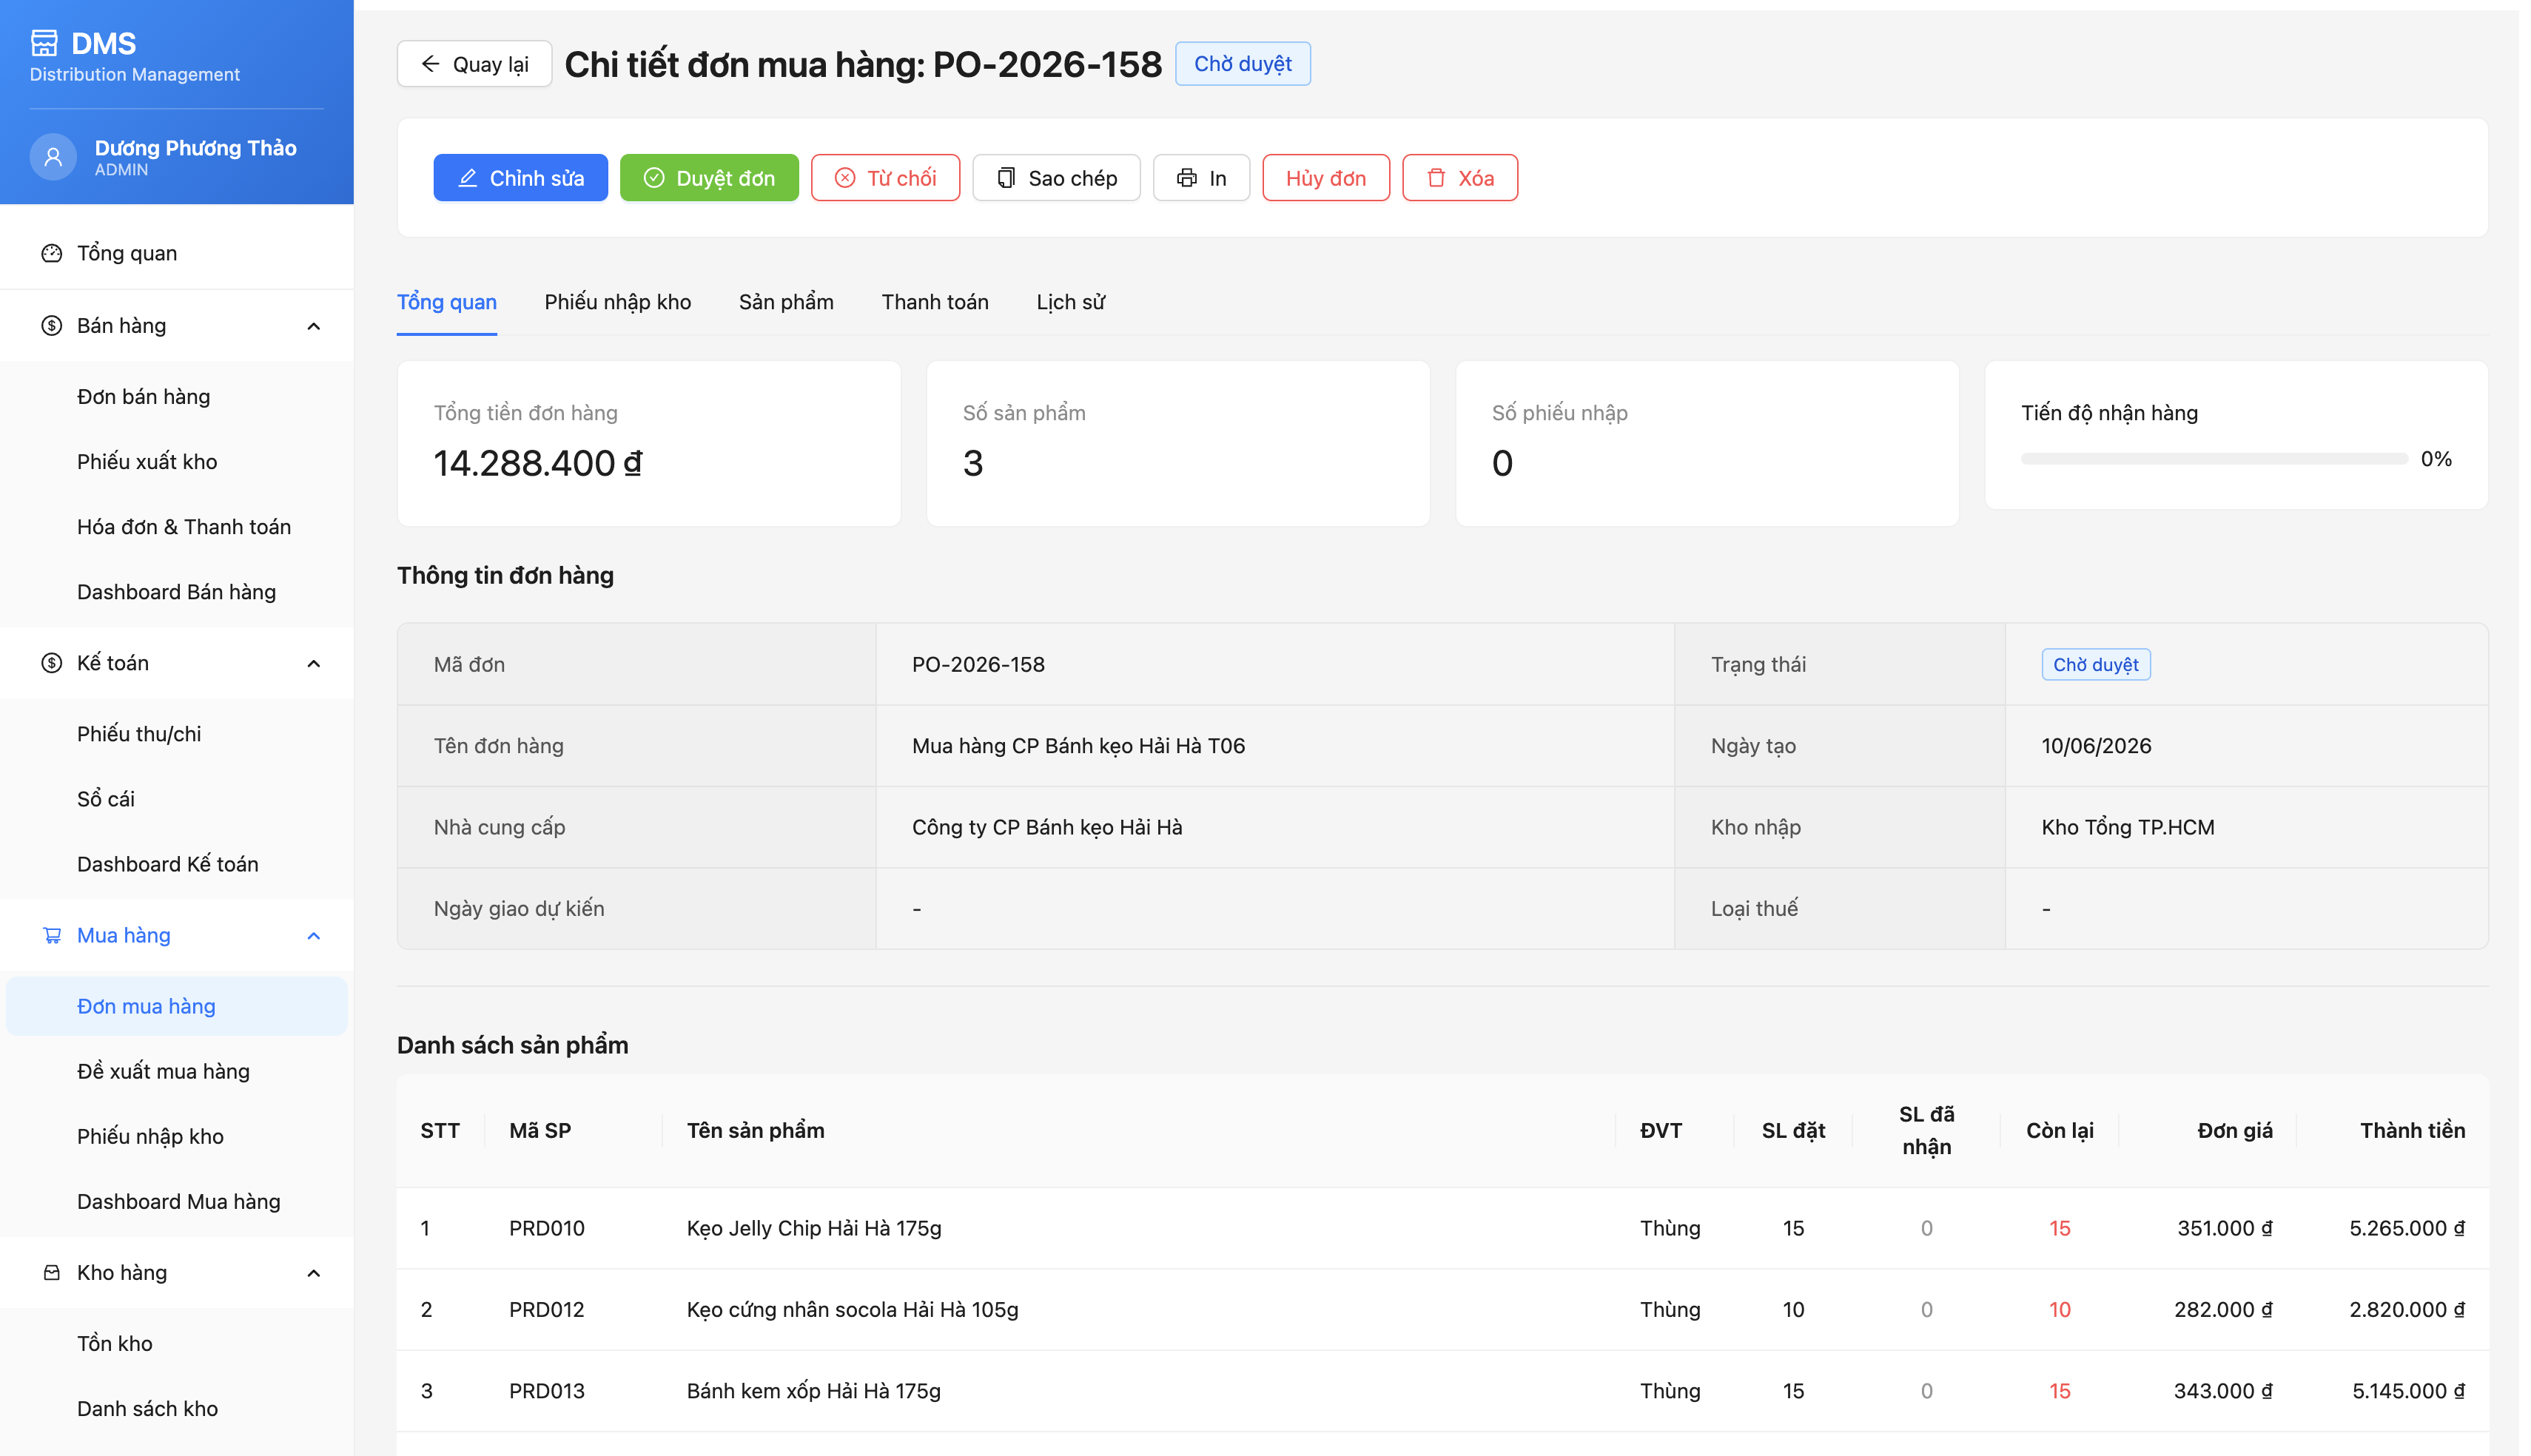
\includegraphics[width=0.95\linewidth]{Figure/screenshots/03-approve-po.png}
\caption{Purchase-order approval}\label{fig:ui-po}
\end{figure}

Figure~\ref{fig:ui-po} shows the detail of purchase order PO-2026-158 in the
pending-approval state, together with its supplier and three ordered lines. The
Approve action visible at the top transitions the order into an approved state
that authorises a subsequent goods receipt; rejecting or editing the order is
only permitted while it remains pending. This screen is the entry point of the
inbound flow.

\begin{figure}[H]\centering
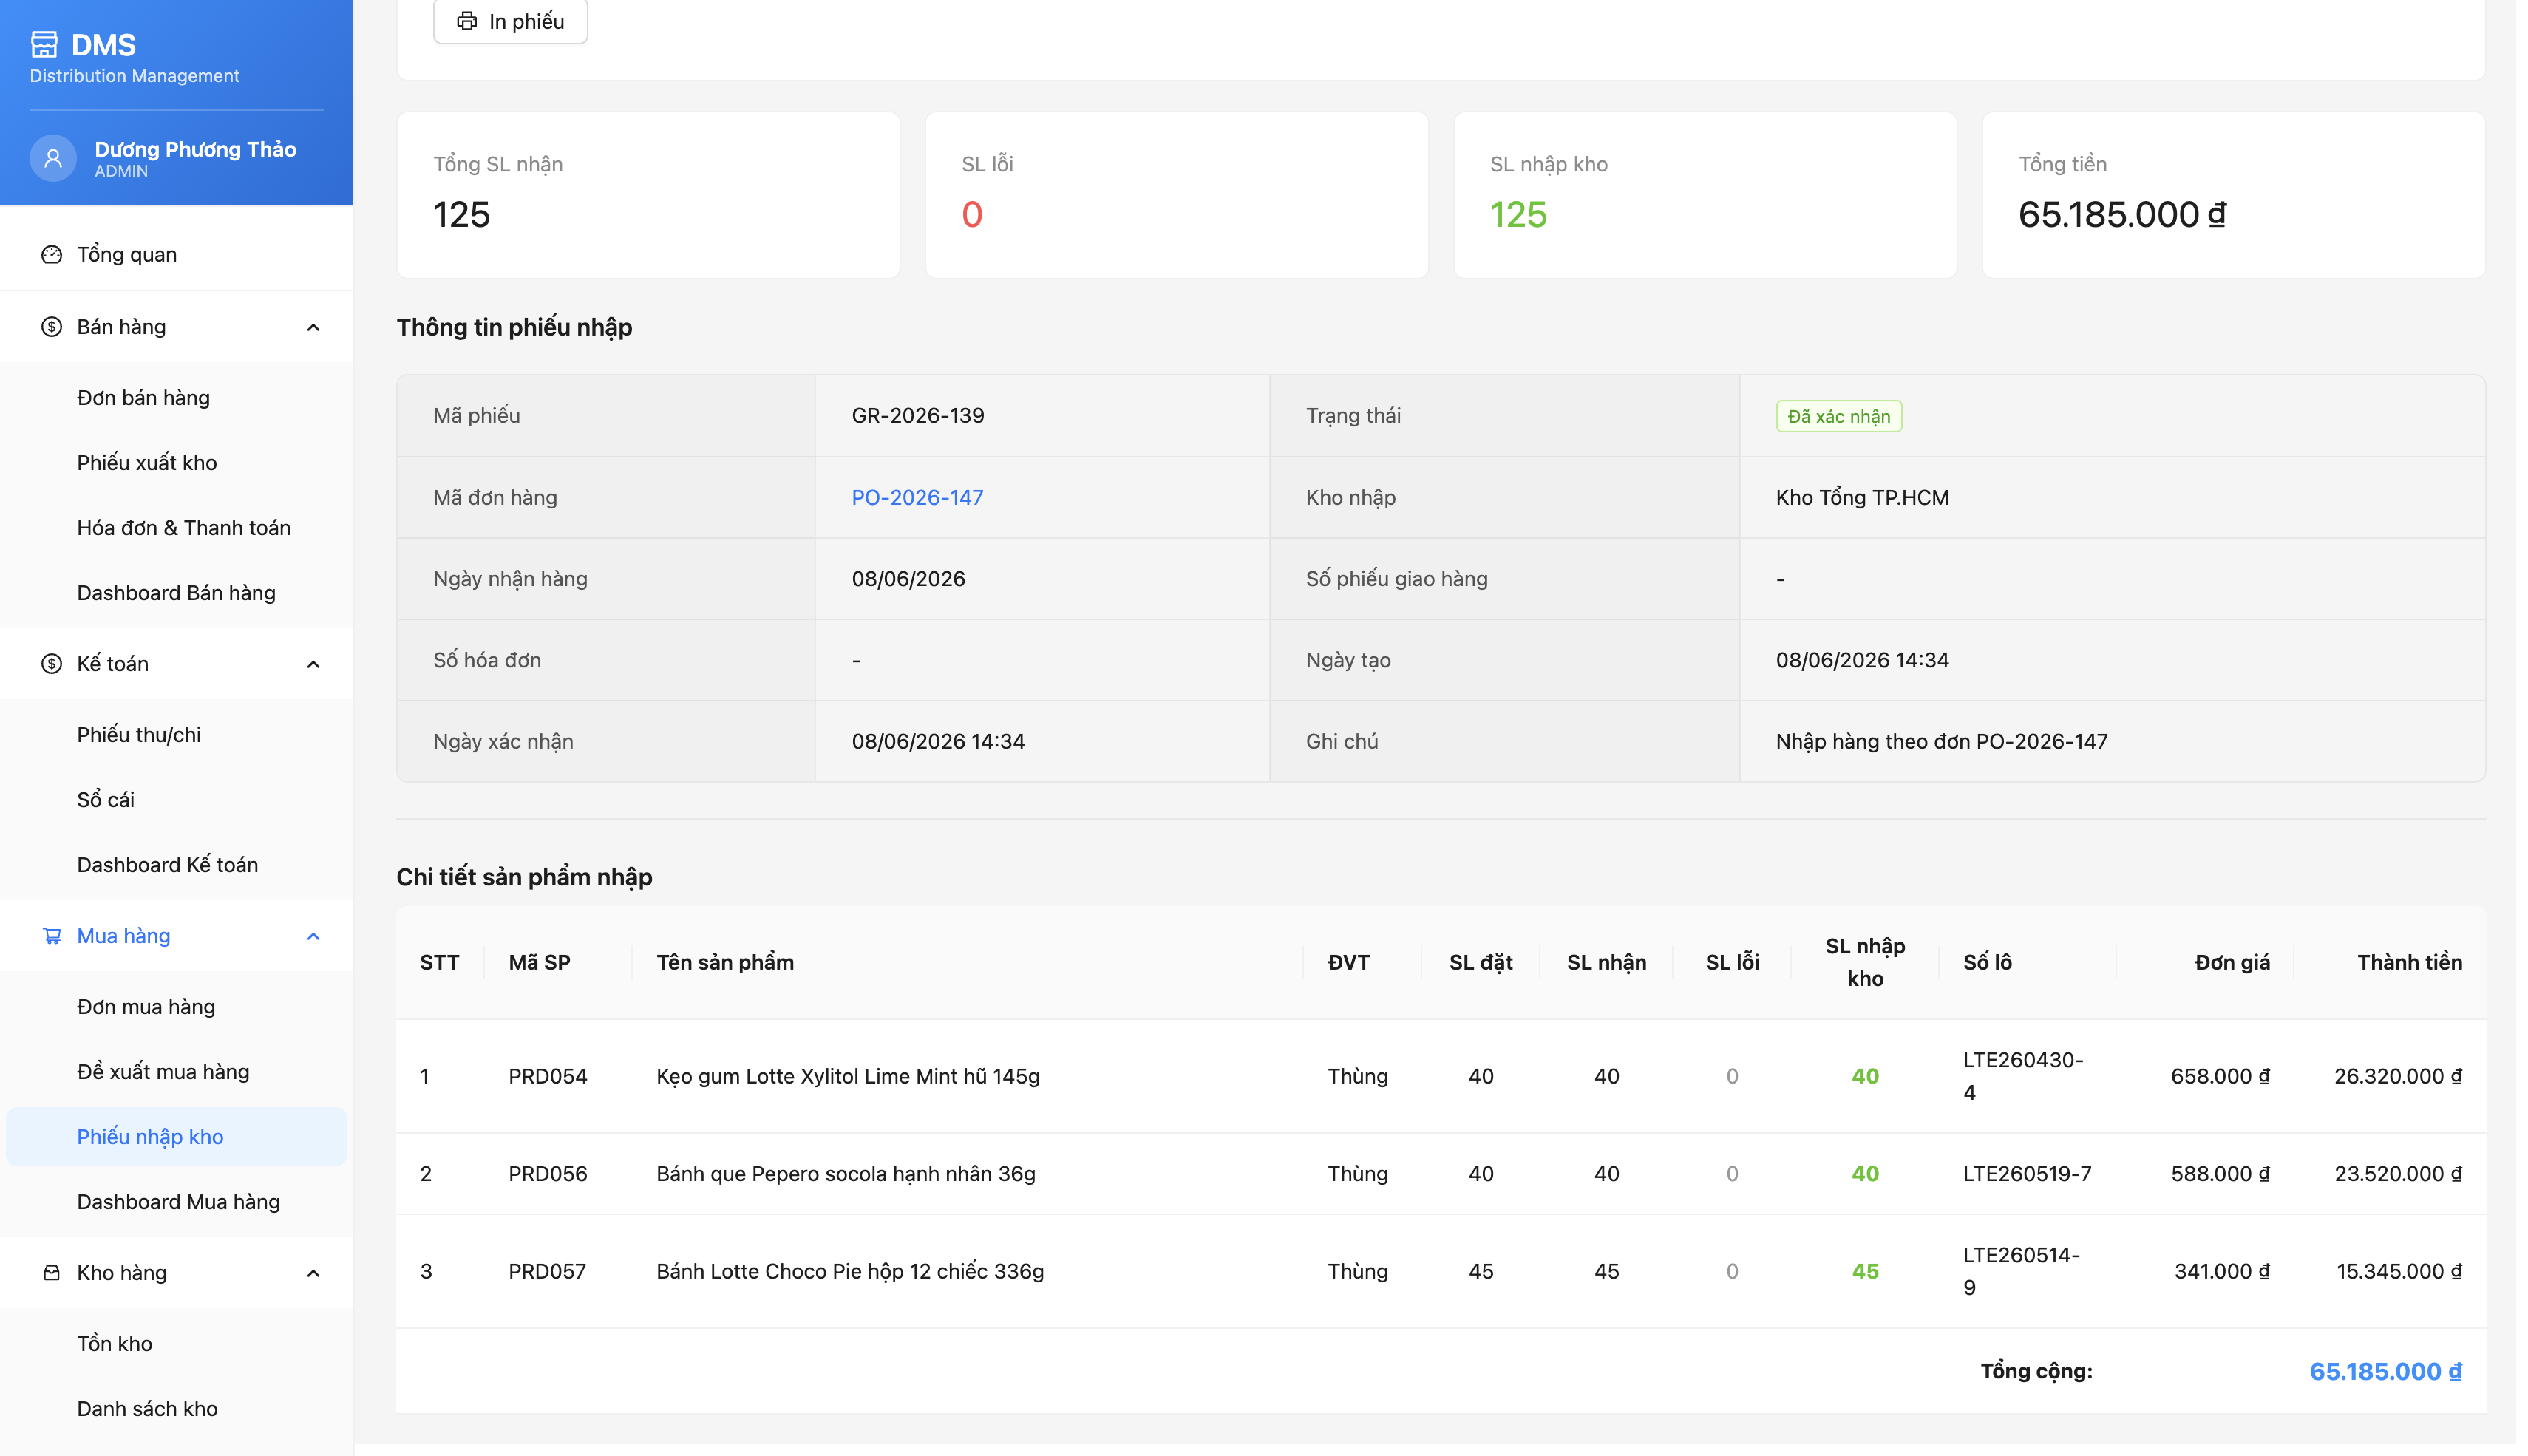
\includegraphics[width=0.95\linewidth]{Figure/screenshots/04-goods-receipt.png}
\caption{Goods-receipt confirmation with per-line lot numbers}\label{fig:ui-gr}
\end{figure}

Figure~\ref{fig:ui-gr} shows the confirmation of goods receipt GR-2026-139 against
purchase order PO-2026-147. Each received line is recorded against a distinct lot
number (for example LTE260430-4), and the accepted quantity is what is finally
added to stock. It is at this point that batch identity enters the system, which
is the precondition for the first-expired-first-out issuing illustrated later in
Figure~\ref{fig:ui-gi} and detailed in the sequence diagram of
Figure~\ref{fig:seq-fefo}.

\begin{figure}[H]\centering
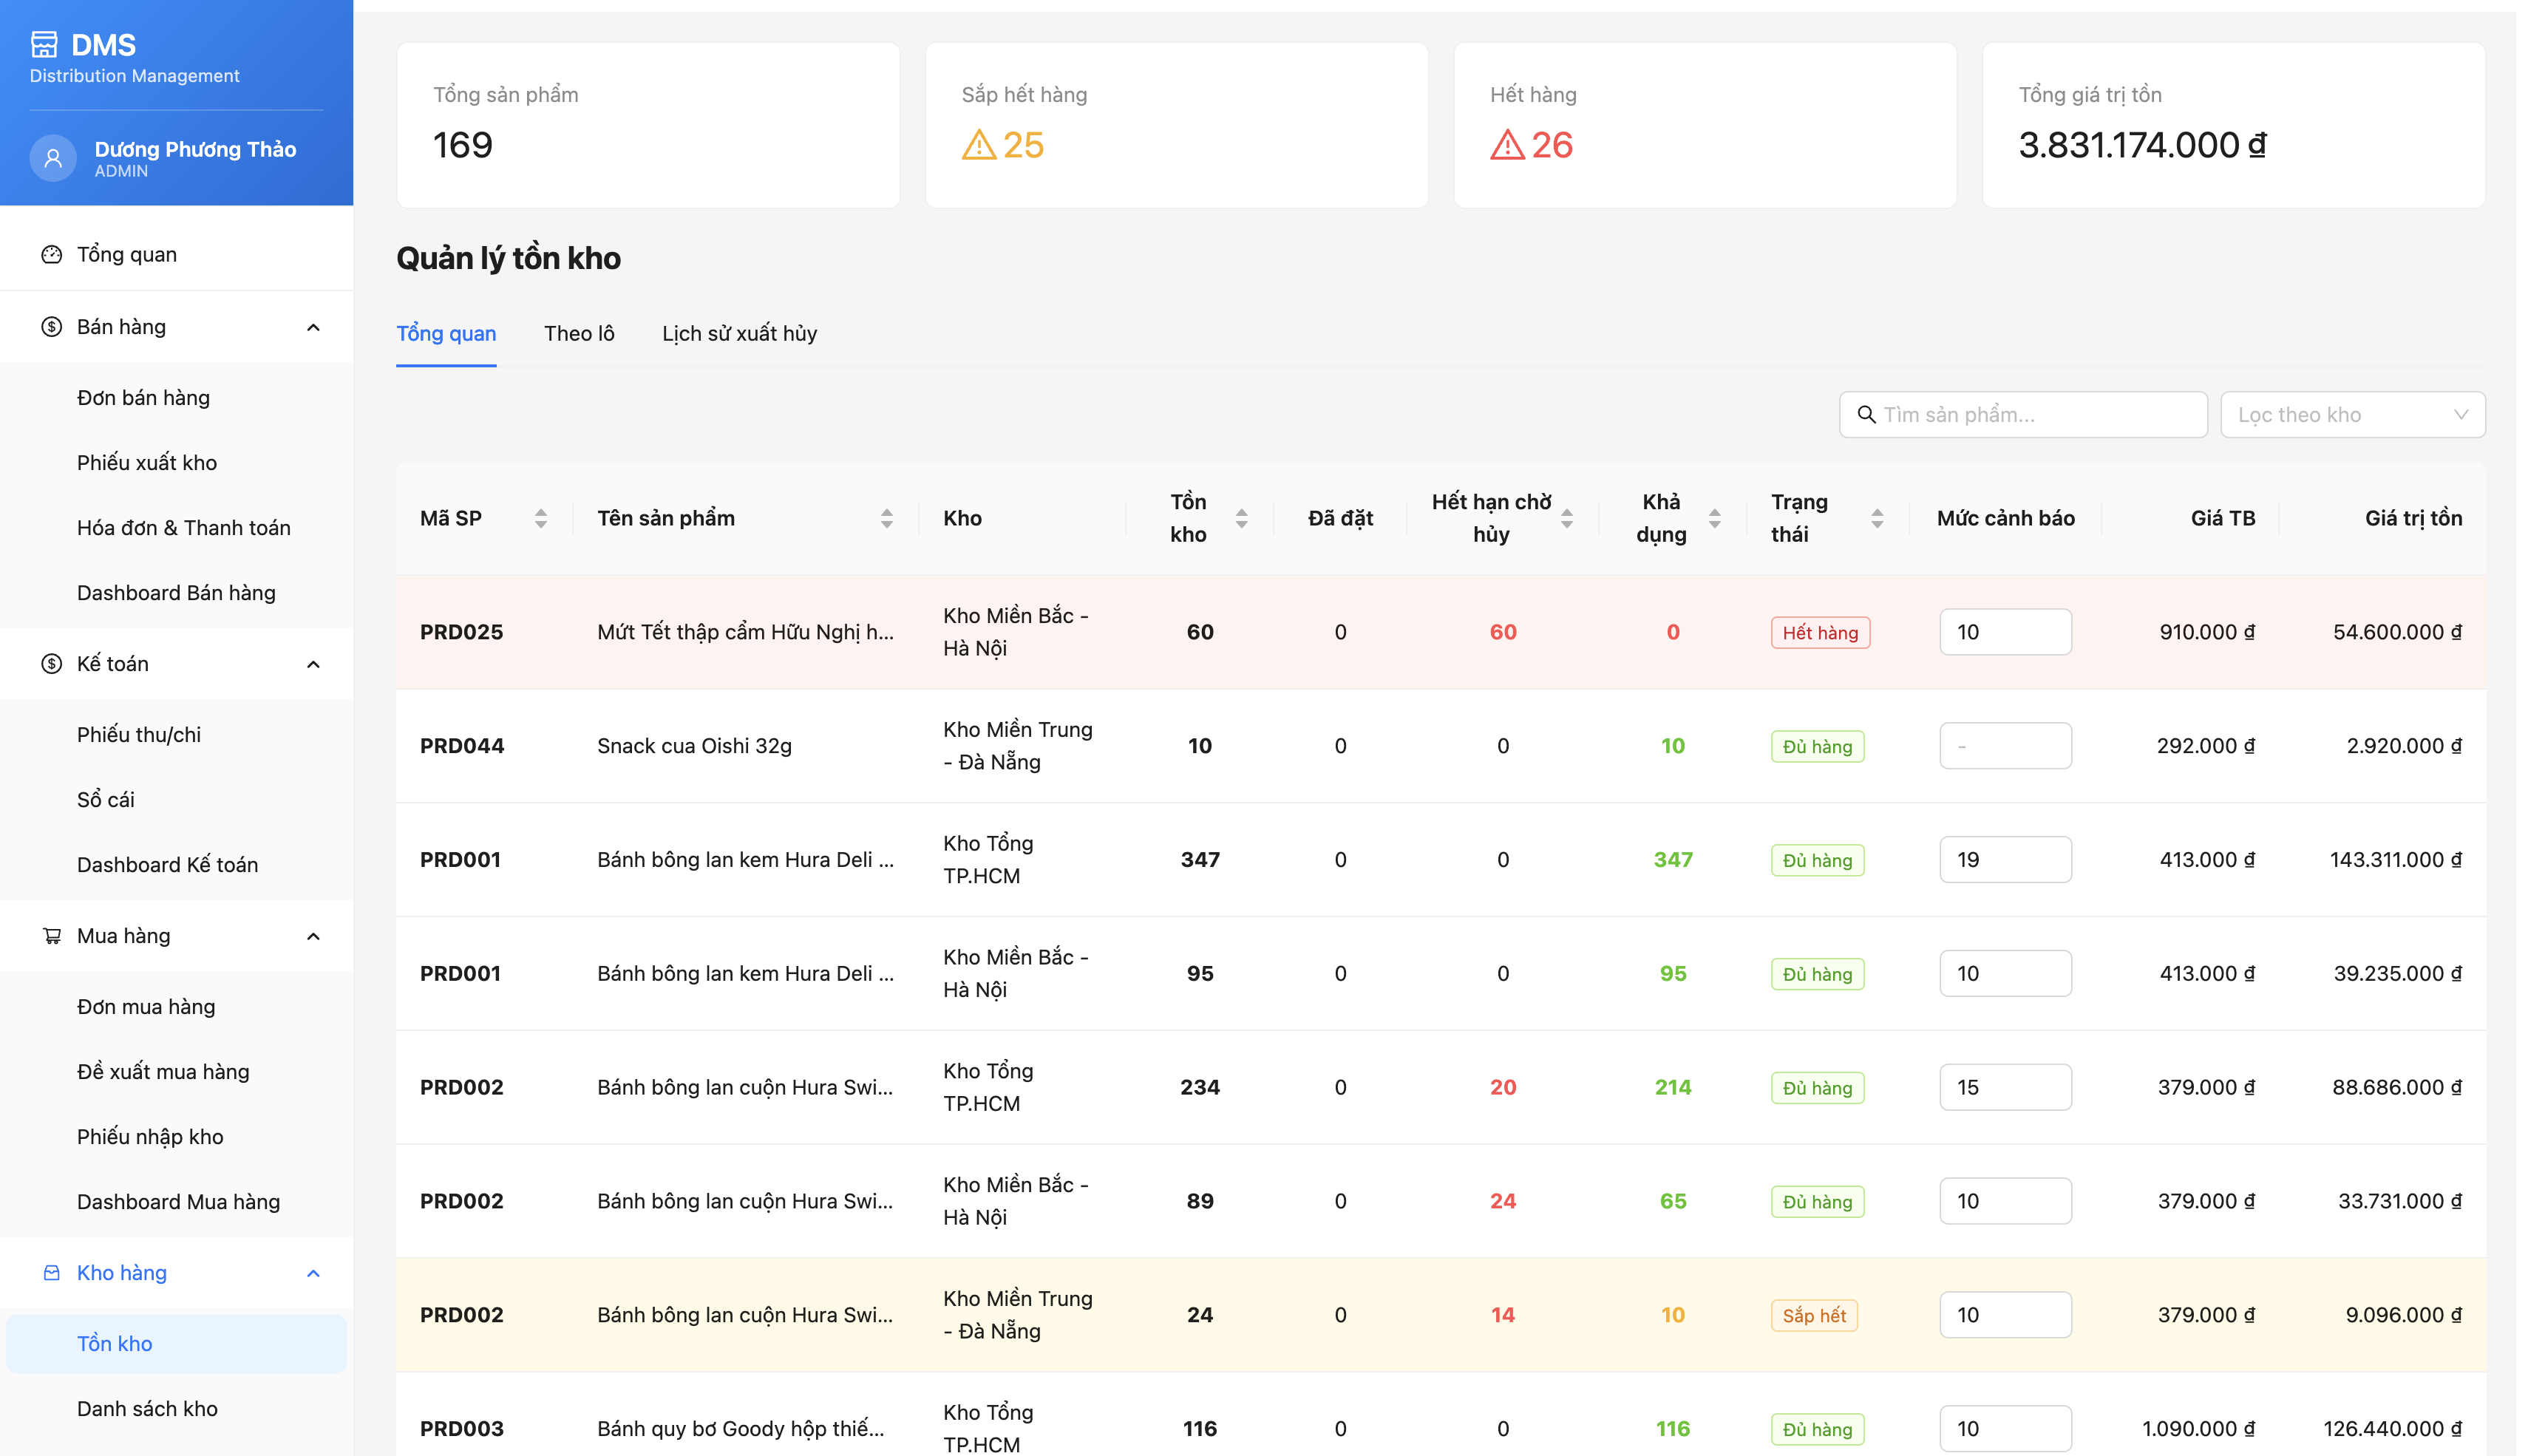
\includegraphics[width=0.95\linewidth]{Figure/screenshots/05-inventory-by-lot.png}
\caption{Inventory overview: on-hand, reserved, available and expiry-pending
quantities per product and warehouse}\label{fig:ui-inventory}
\end{figure}

Figure~\ref{fig:ui-inventory} shows the inventory overview. For each
product-warehouse pair the table separates quantity on hand, reserved quantity,
quantity pending disposal because of expiry, and available quantity, and assigns
a status tag such as in-stock, low-stock, or out-of-stock. This separation is the
on-screen manifestation of the reservation mechanism: the available quantity is
computed as the quantity on hand minus the reserved quantity, and it is this
available figure, not the raw on-hand figure, that is checked when a sales order
is approved. Confirming a goods issue is what finally lowers the on-hand quantity.

\begin{figure}[H]\centering
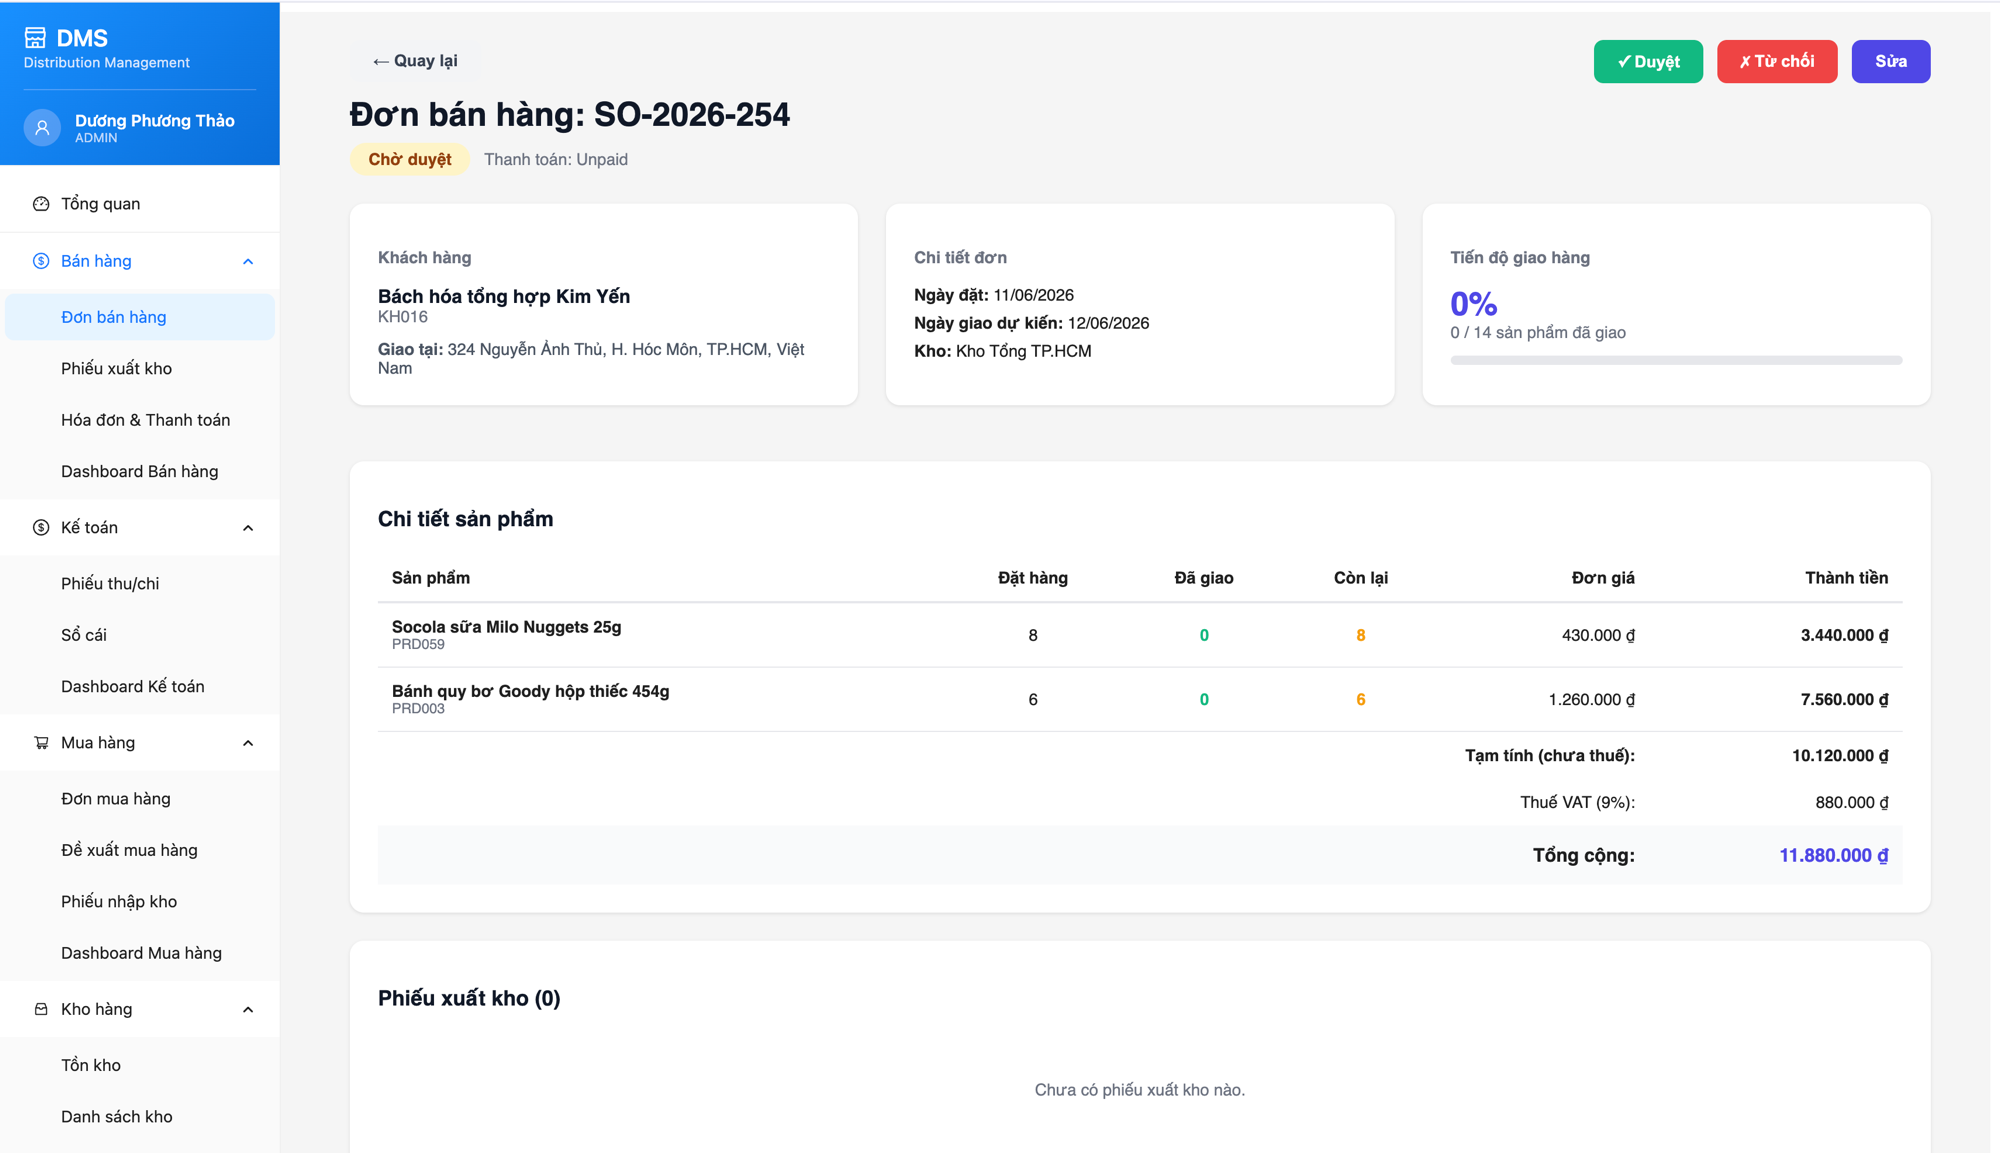
\includegraphics[width=0.95\linewidth]{Figure/screenshots/06-approve-so.png}
\caption{Sales-order approval, the point at which available stock is checked and
reserved}\label{fig:ui-so}
\end{figure}

Figure~\ref{fig:ui-so} shows sales order SO-2026-254 in the pending-approval
state, with its customer, two ordered lines, and the computed subtotal, value-added
tax, and total. Approval is the decisive step in the outbound flow: when the
Approve action is invoked, the server checks that sufficient available stock
exists for every line and, if so, reserves exactly the ordered quantity before
moving the order to the approved state. This is where the available-quantity logic
visible in Figure~\ref{fig:ui-inventory} is enforced, so that two orders competing
for the same stock cannot both be approved beyond what is physically on hand. The
delivery-progress indicator remains at zero per cent until the corresponding goods
issue is confirmed.

\begin{figure}[H]\centering
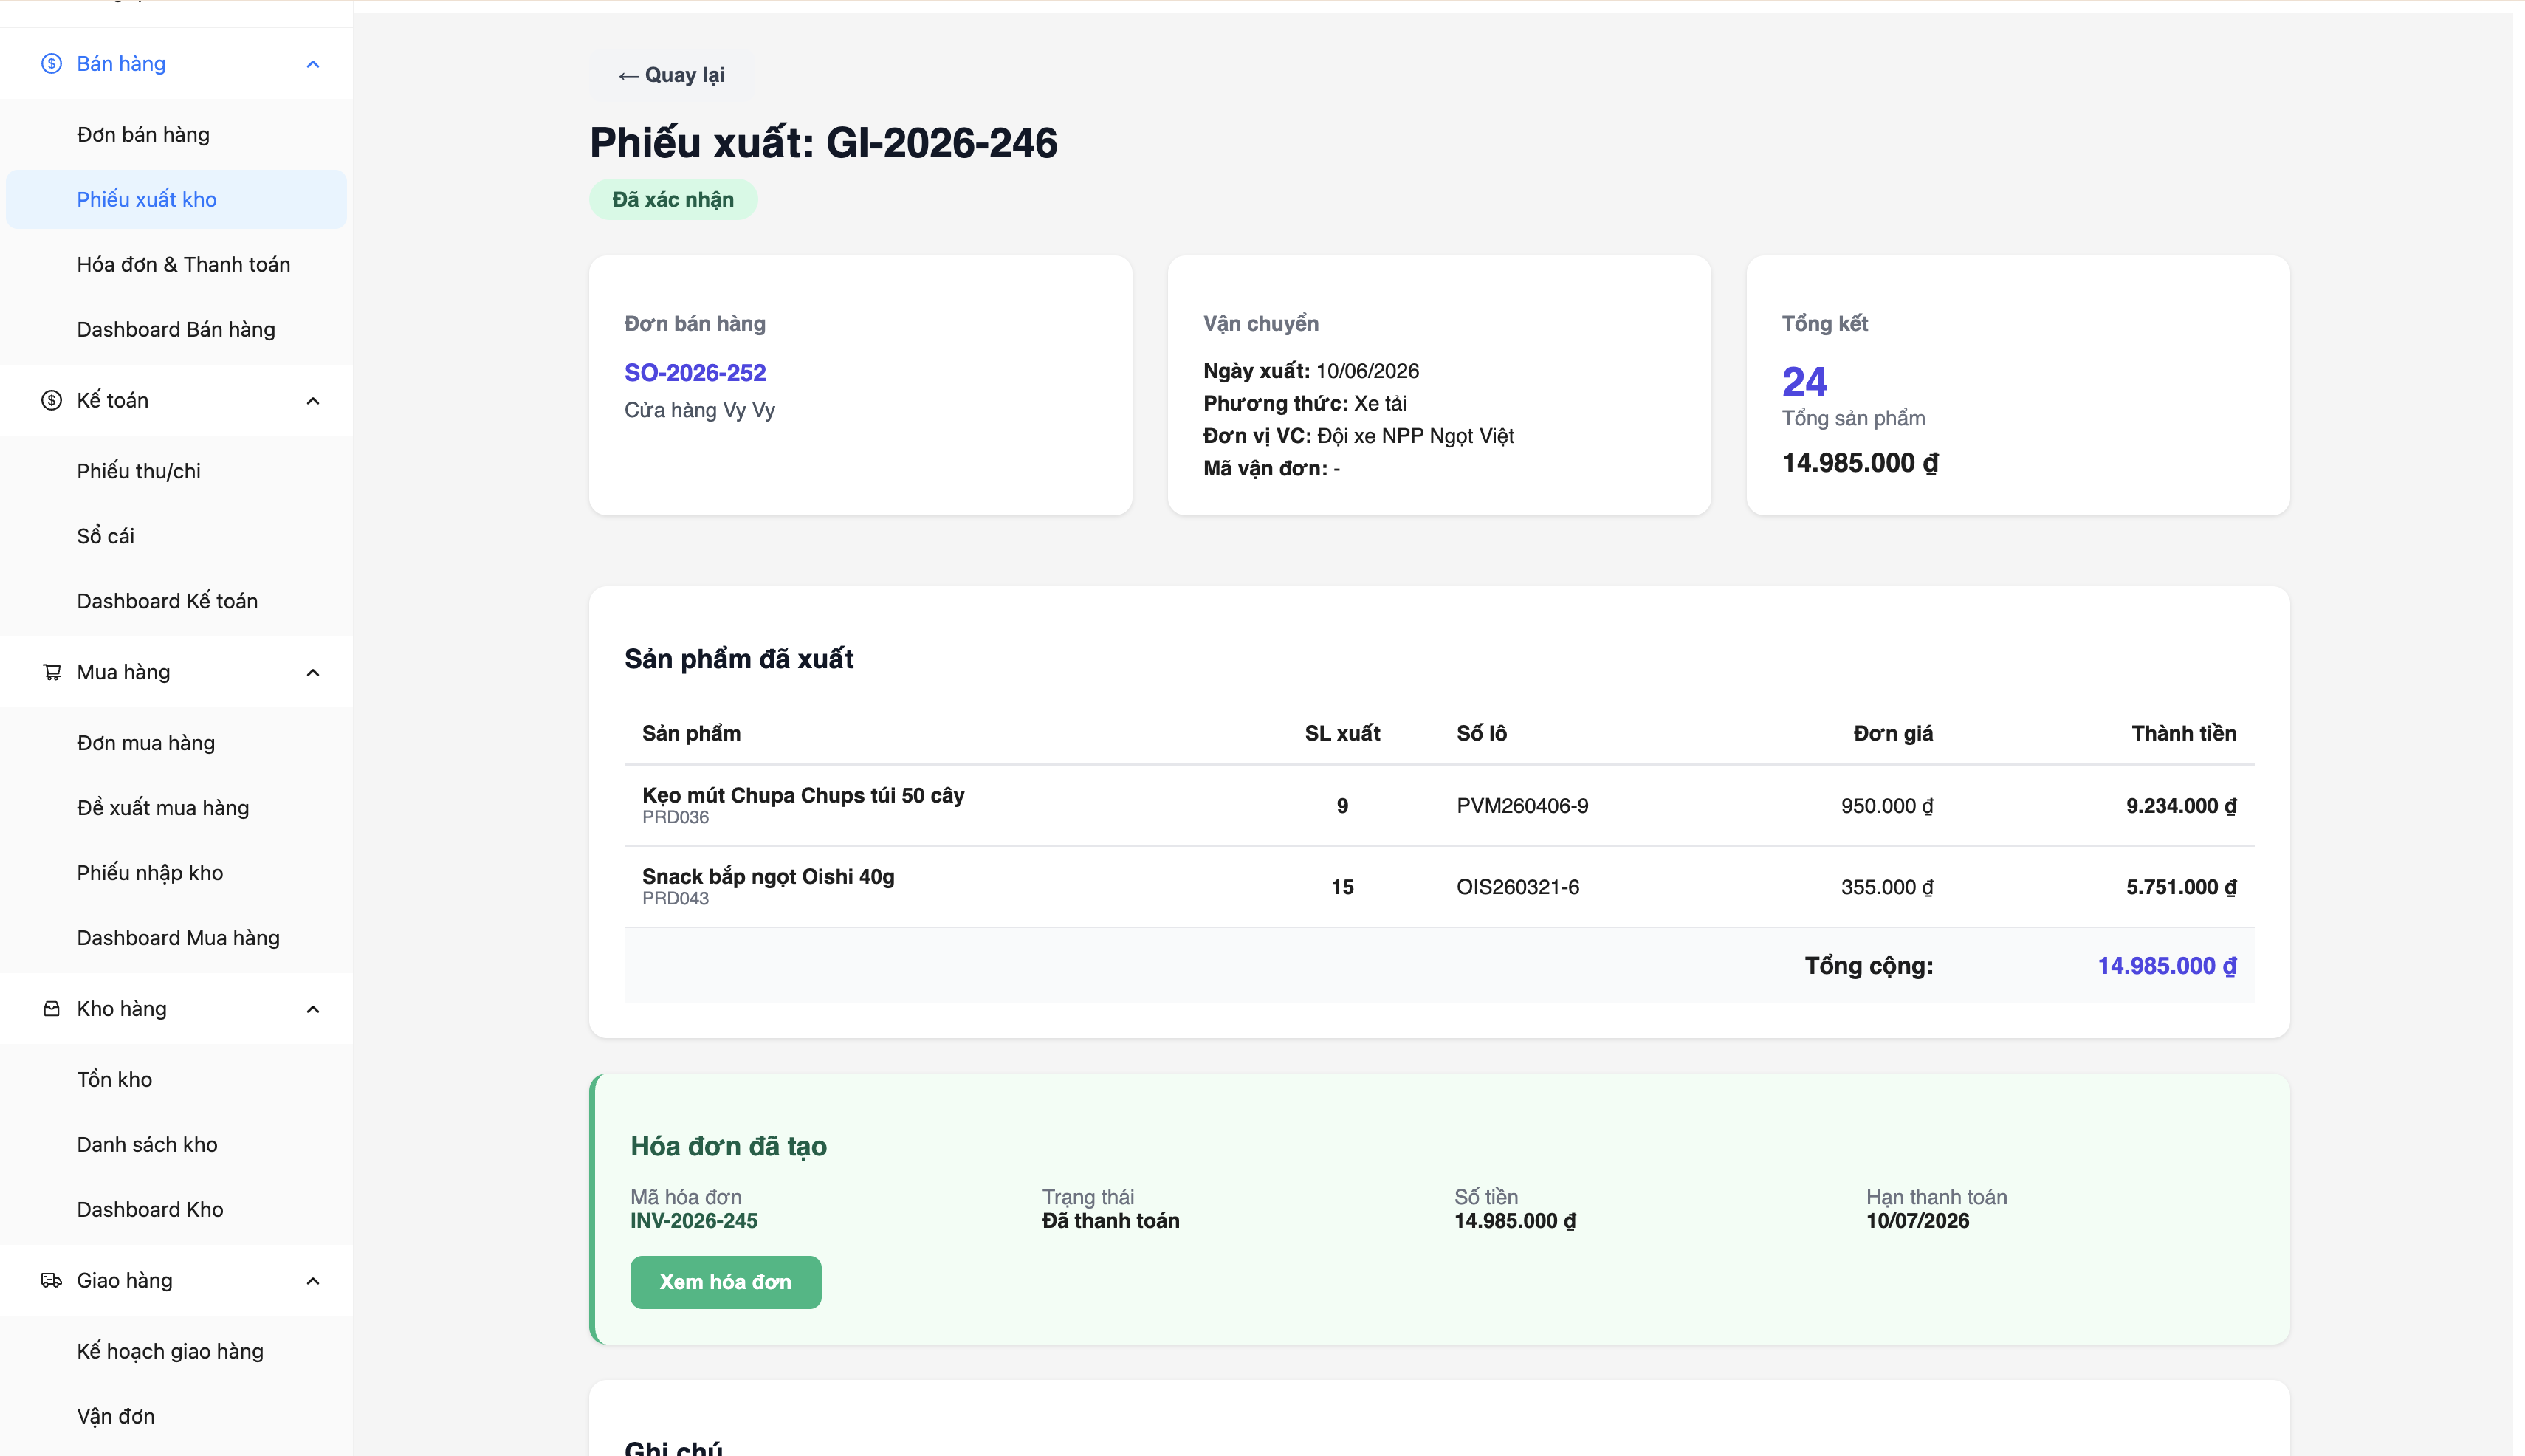
\includegraphics[width=0.95\linewidth]{Figure/screenshots/07-goods-issue-fefo.png}
\caption{Goods-issue confirmation with FEFO lot allocation}\label{fig:ui-gi}
\end{figure}

Figure~\ref{fig:ui-gi} shows the confirmation of goods issue GI-2026-246, which
fulfils sales order SO-2026-252. Each issued line is annotated with the specific
lot consumed (for example PVM260406-9), and these lots are the earliest-expiring
ones available, selected automatically by the FEFO allocation query rather than
chosen by the operator. The same panel shows that sales invoice INV-2026-245 is
generated automatically once the issue is confirmed, linking the warehouse and
accounting subsystems in a single transaction.

\begin{figure}[H]\centering
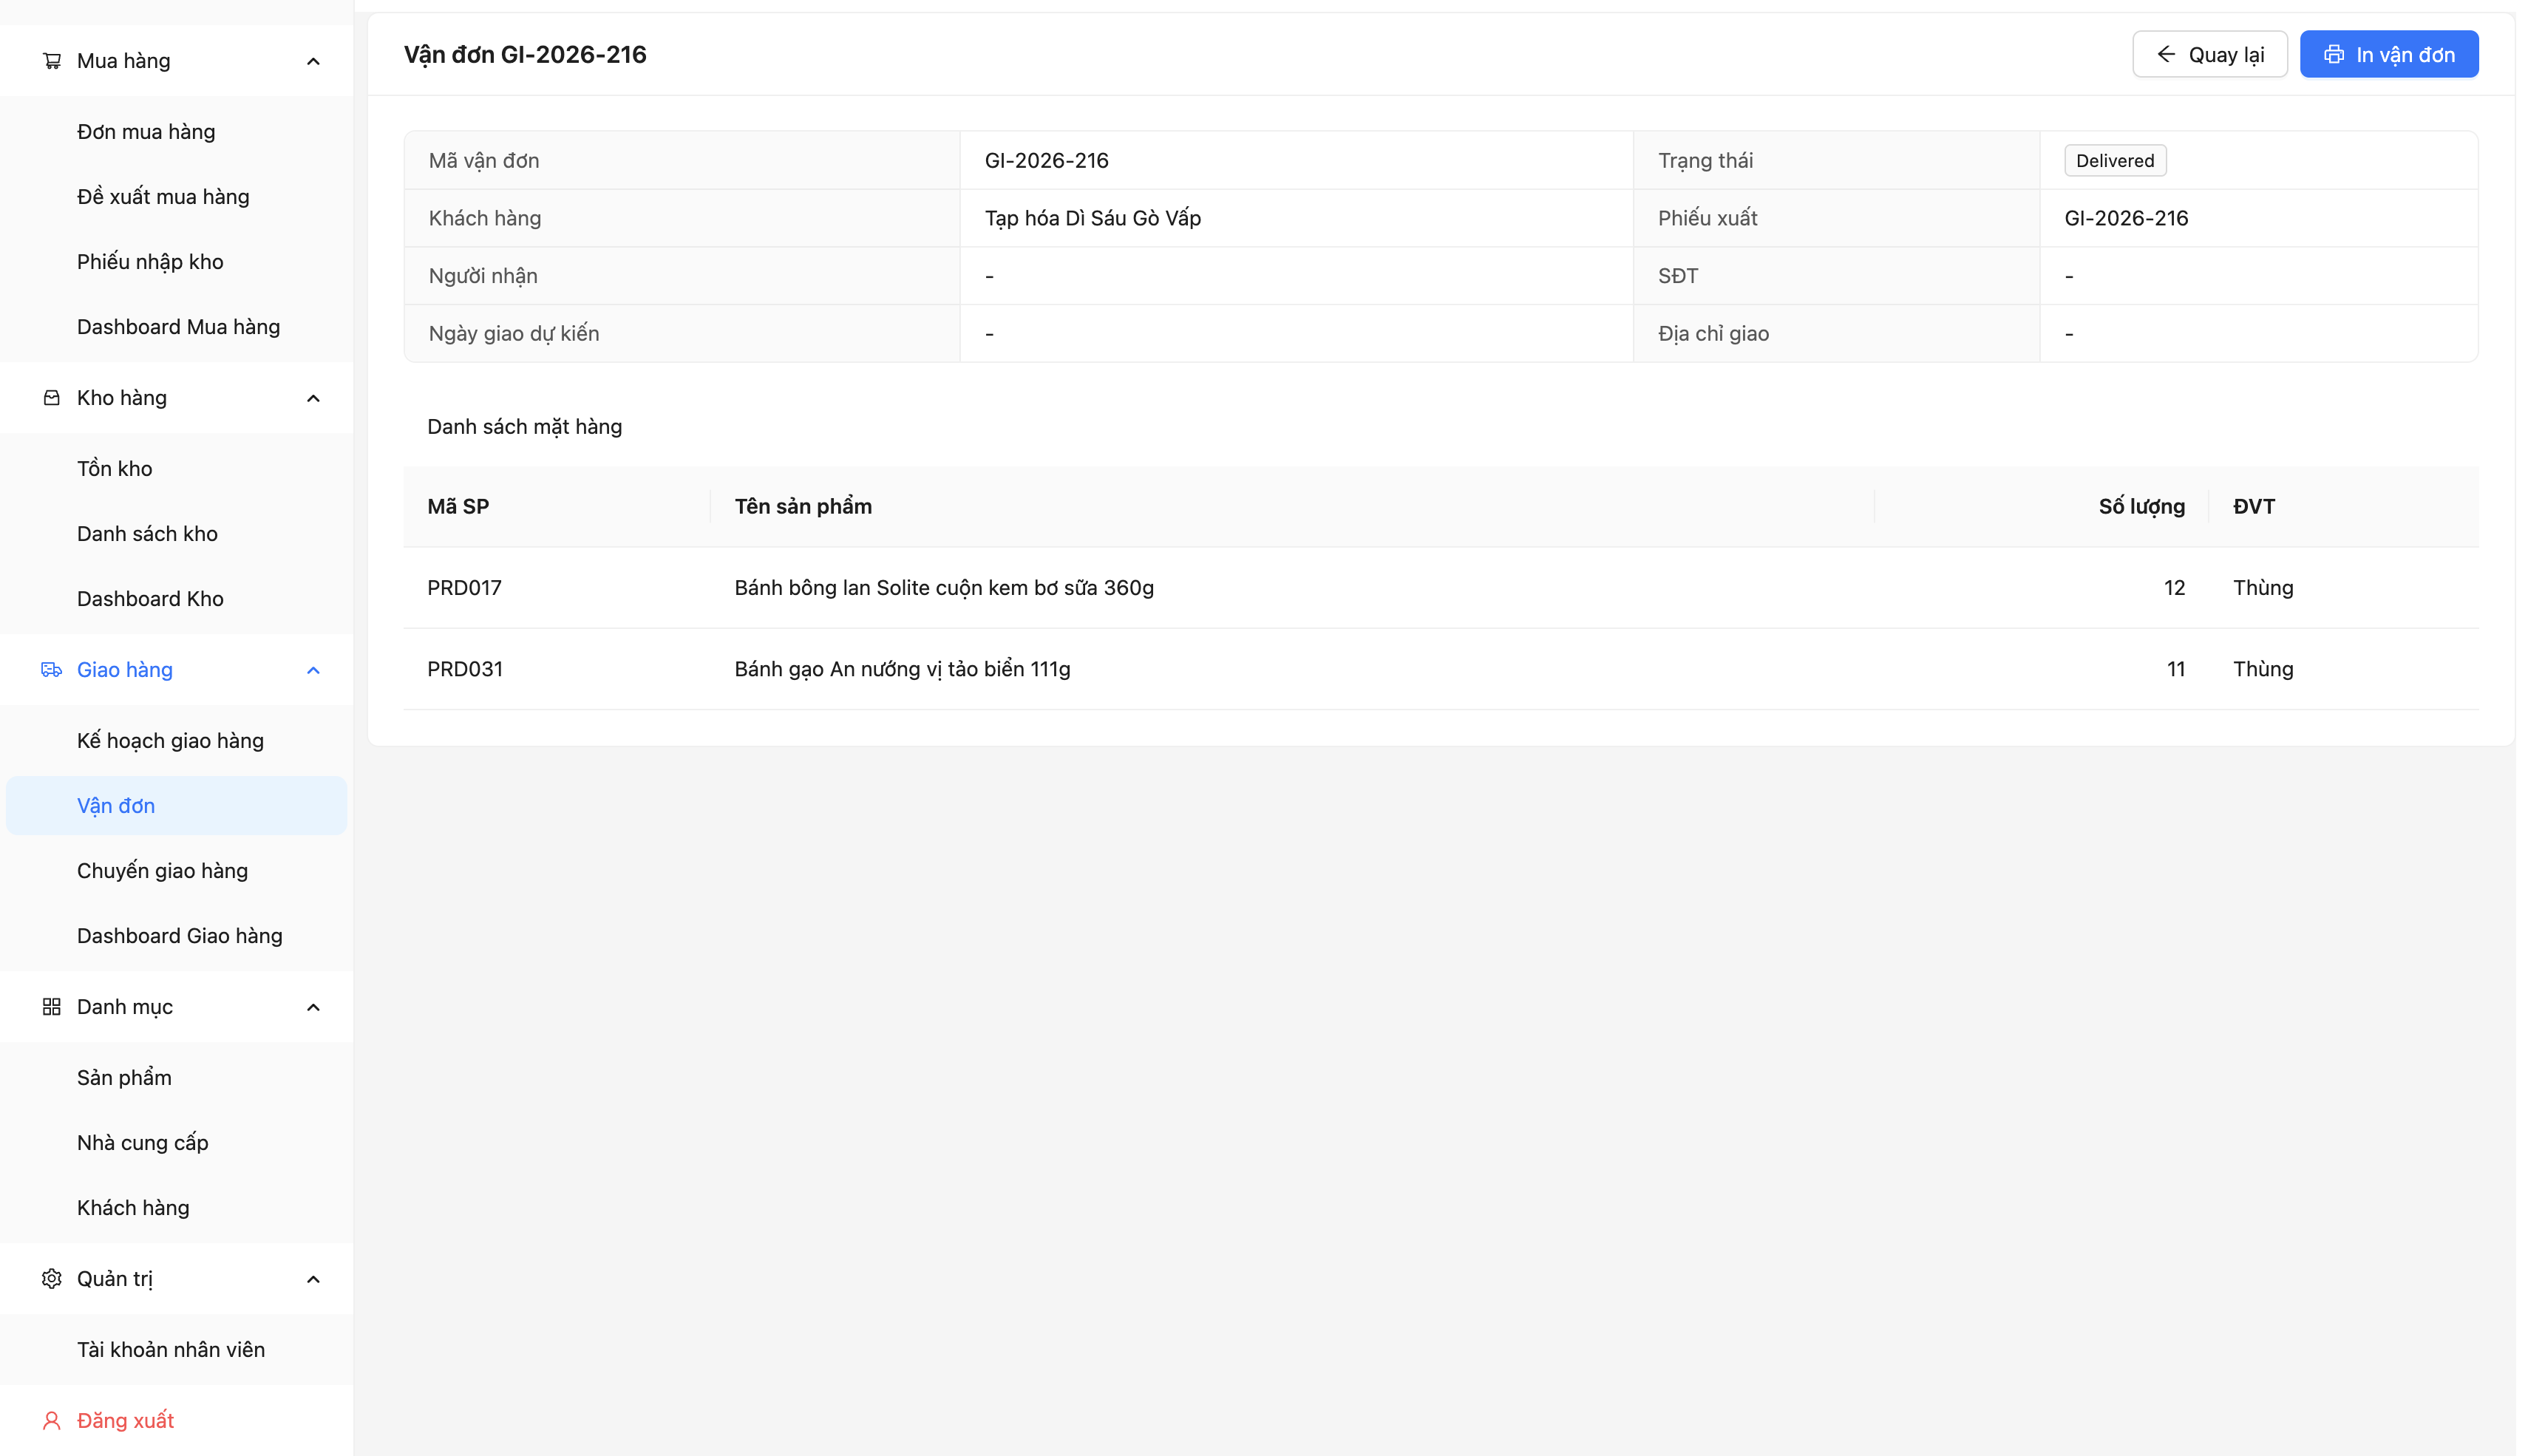
\includegraphics[width=0.95\linewidth]{Figure/screenshots/08-delivery-waybill.png}
\caption{Delivery waybill in the delivered state}\label{fig:ui-waybill}
\end{figure}

Figure~\ref{fig:ui-waybill} shows the waybill associated with issue GI-2026-216
after the trip has been completed, with its status set to delivered and the two
product lines to be handed to the customer. A printable version of this document
accompanies the driver; when a delivery fails instead of completing, the
corresponding stock is returned to inventory through the failed-delivery recovery
path discussed in Chapter~\ref{chapter:Contribution}.

\begin{figure}[H]\centering
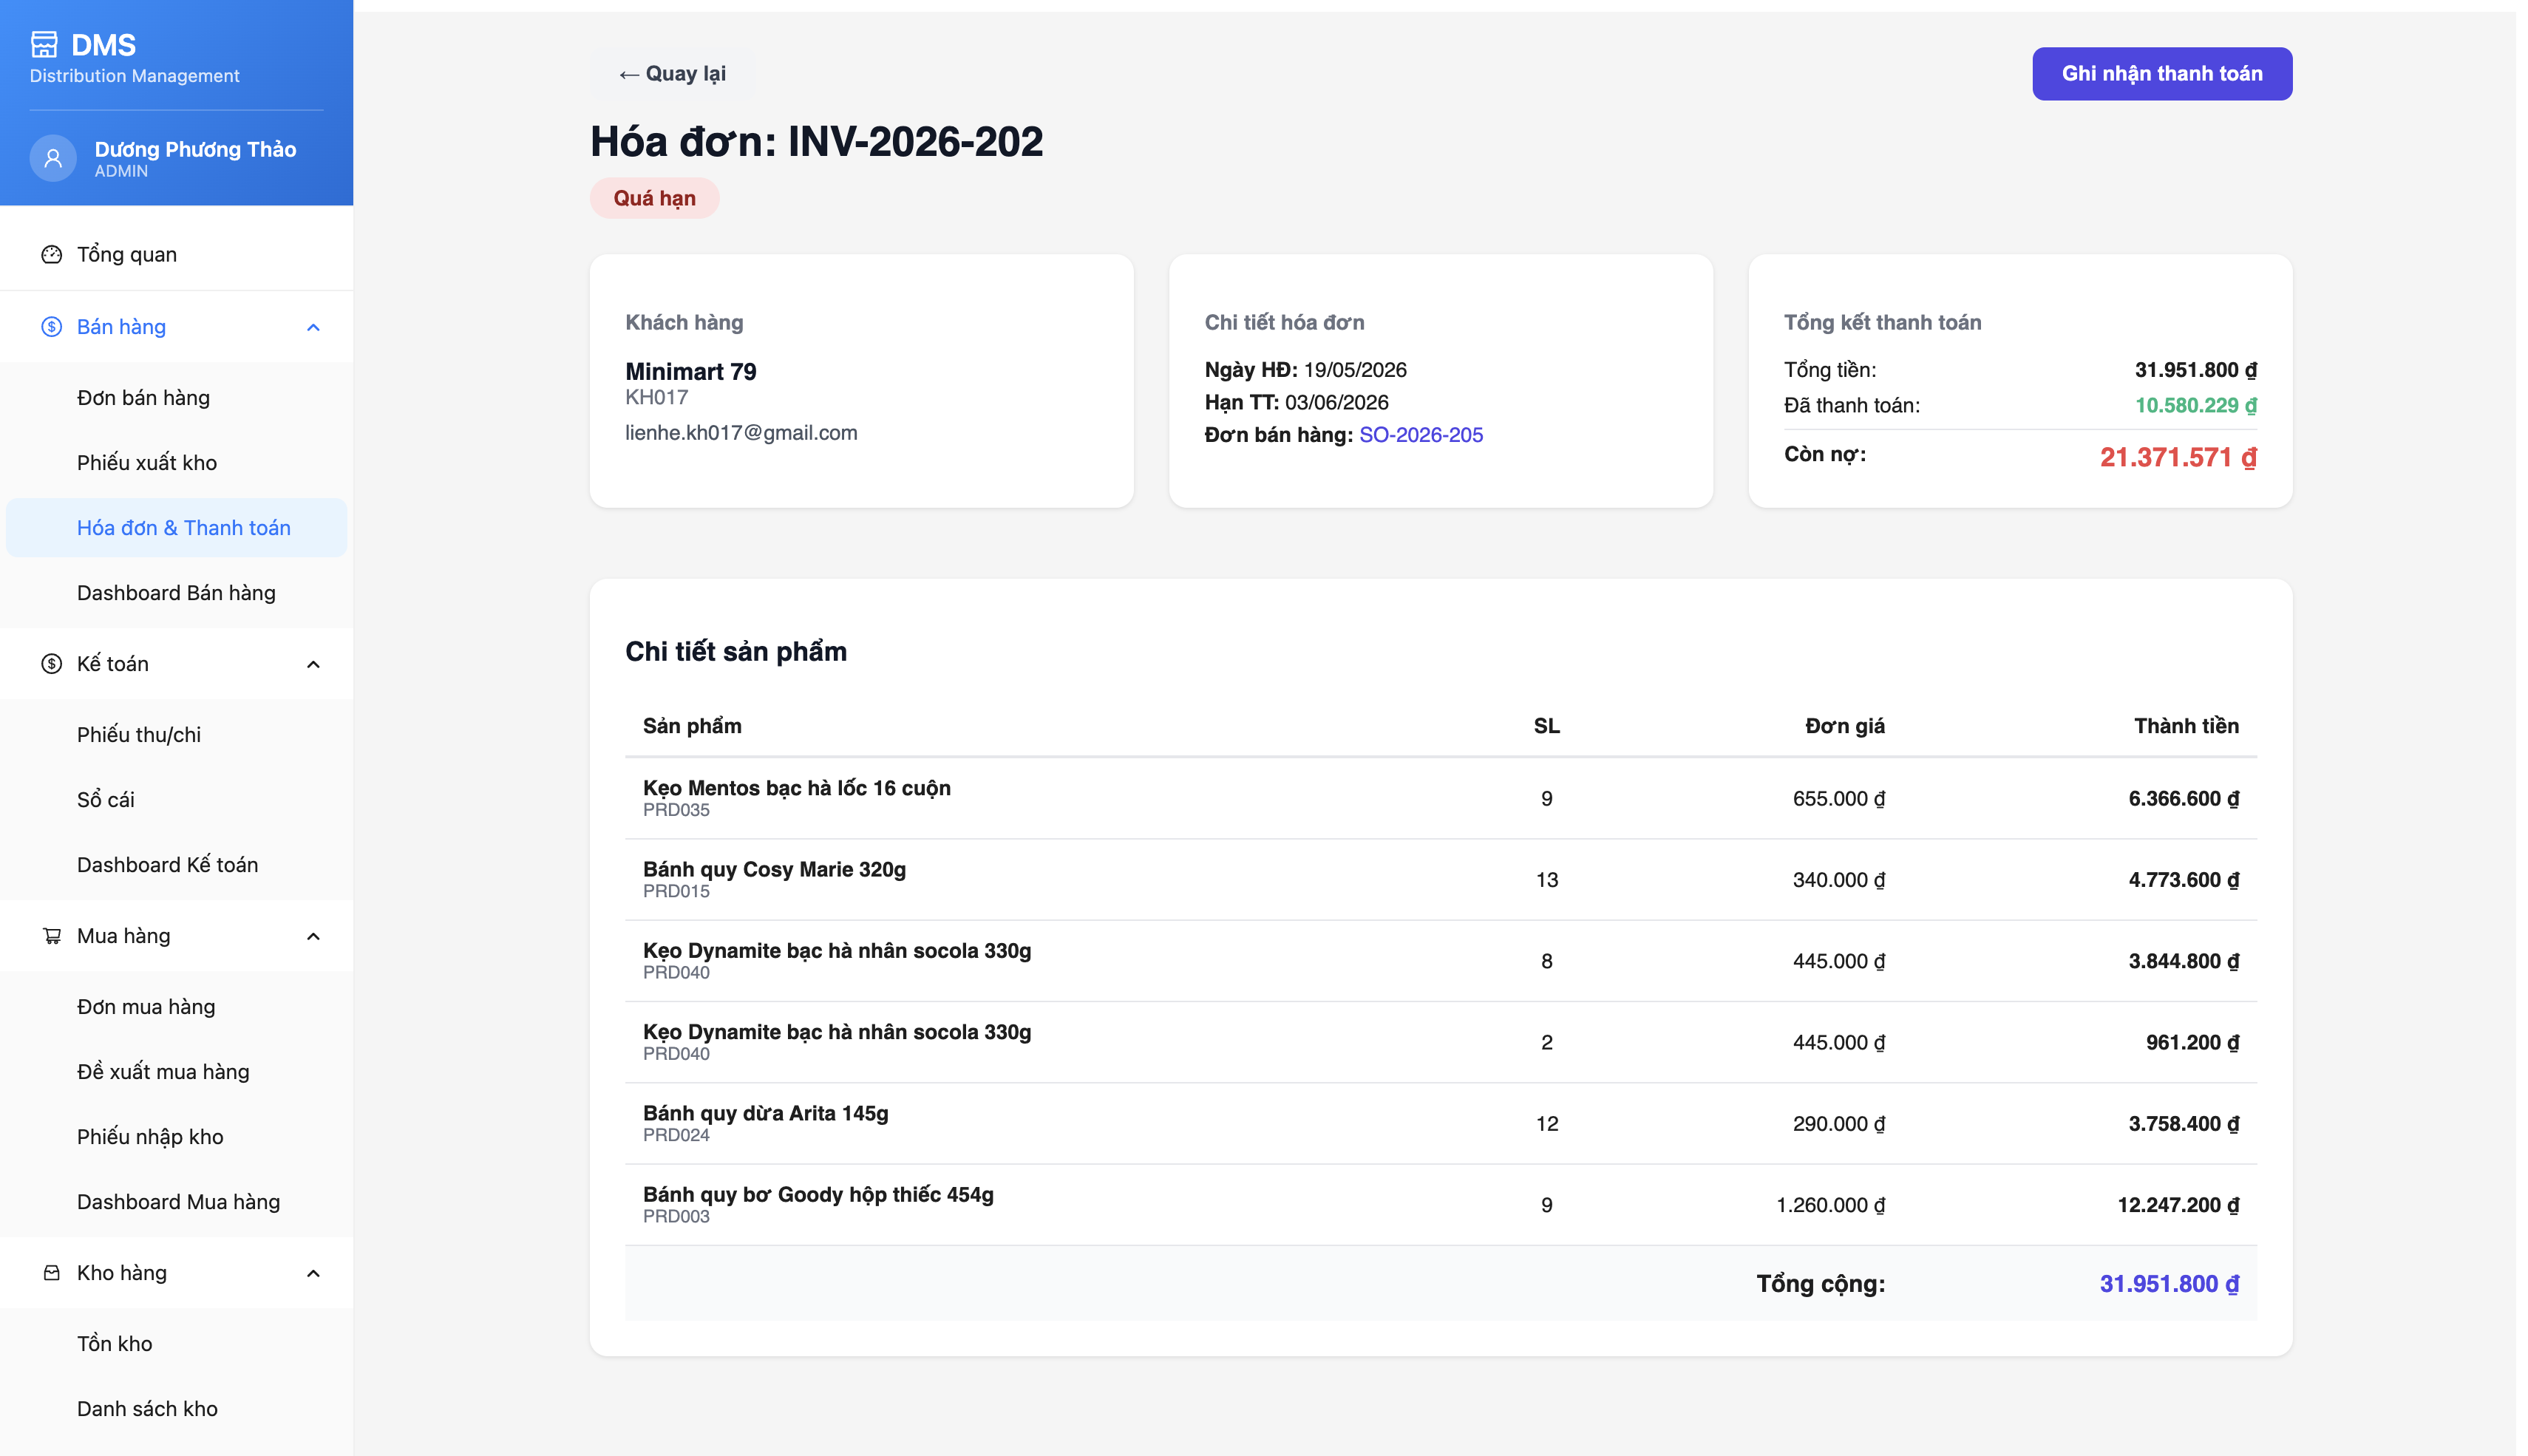
\includegraphics[width=0.95\linewidth]{Figure/screenshots/09-invoice.png}
\caption{Sales-invoice detail with partial settlement}\label{fig:ui-invoice}
\end{figure}

Figure~\ref{fig:ui-invoice} shows sales invoice INV-2026-202, issued to customer
Minimart~79 from sales order SO-2026-205. The invoice is only partially settled:
of a total of 31{,}951{,}800~VND, 10{,}580{,}229~VND has been received, leaving
21{,}371{,}571~VND outstanding, and the invoice is consequently flagged as
overdue. This partial-payment state is what the receivables ledger in
Figure~\ref{fig:ui-ledger} reconciles.

\begin{figure}[H]\centering
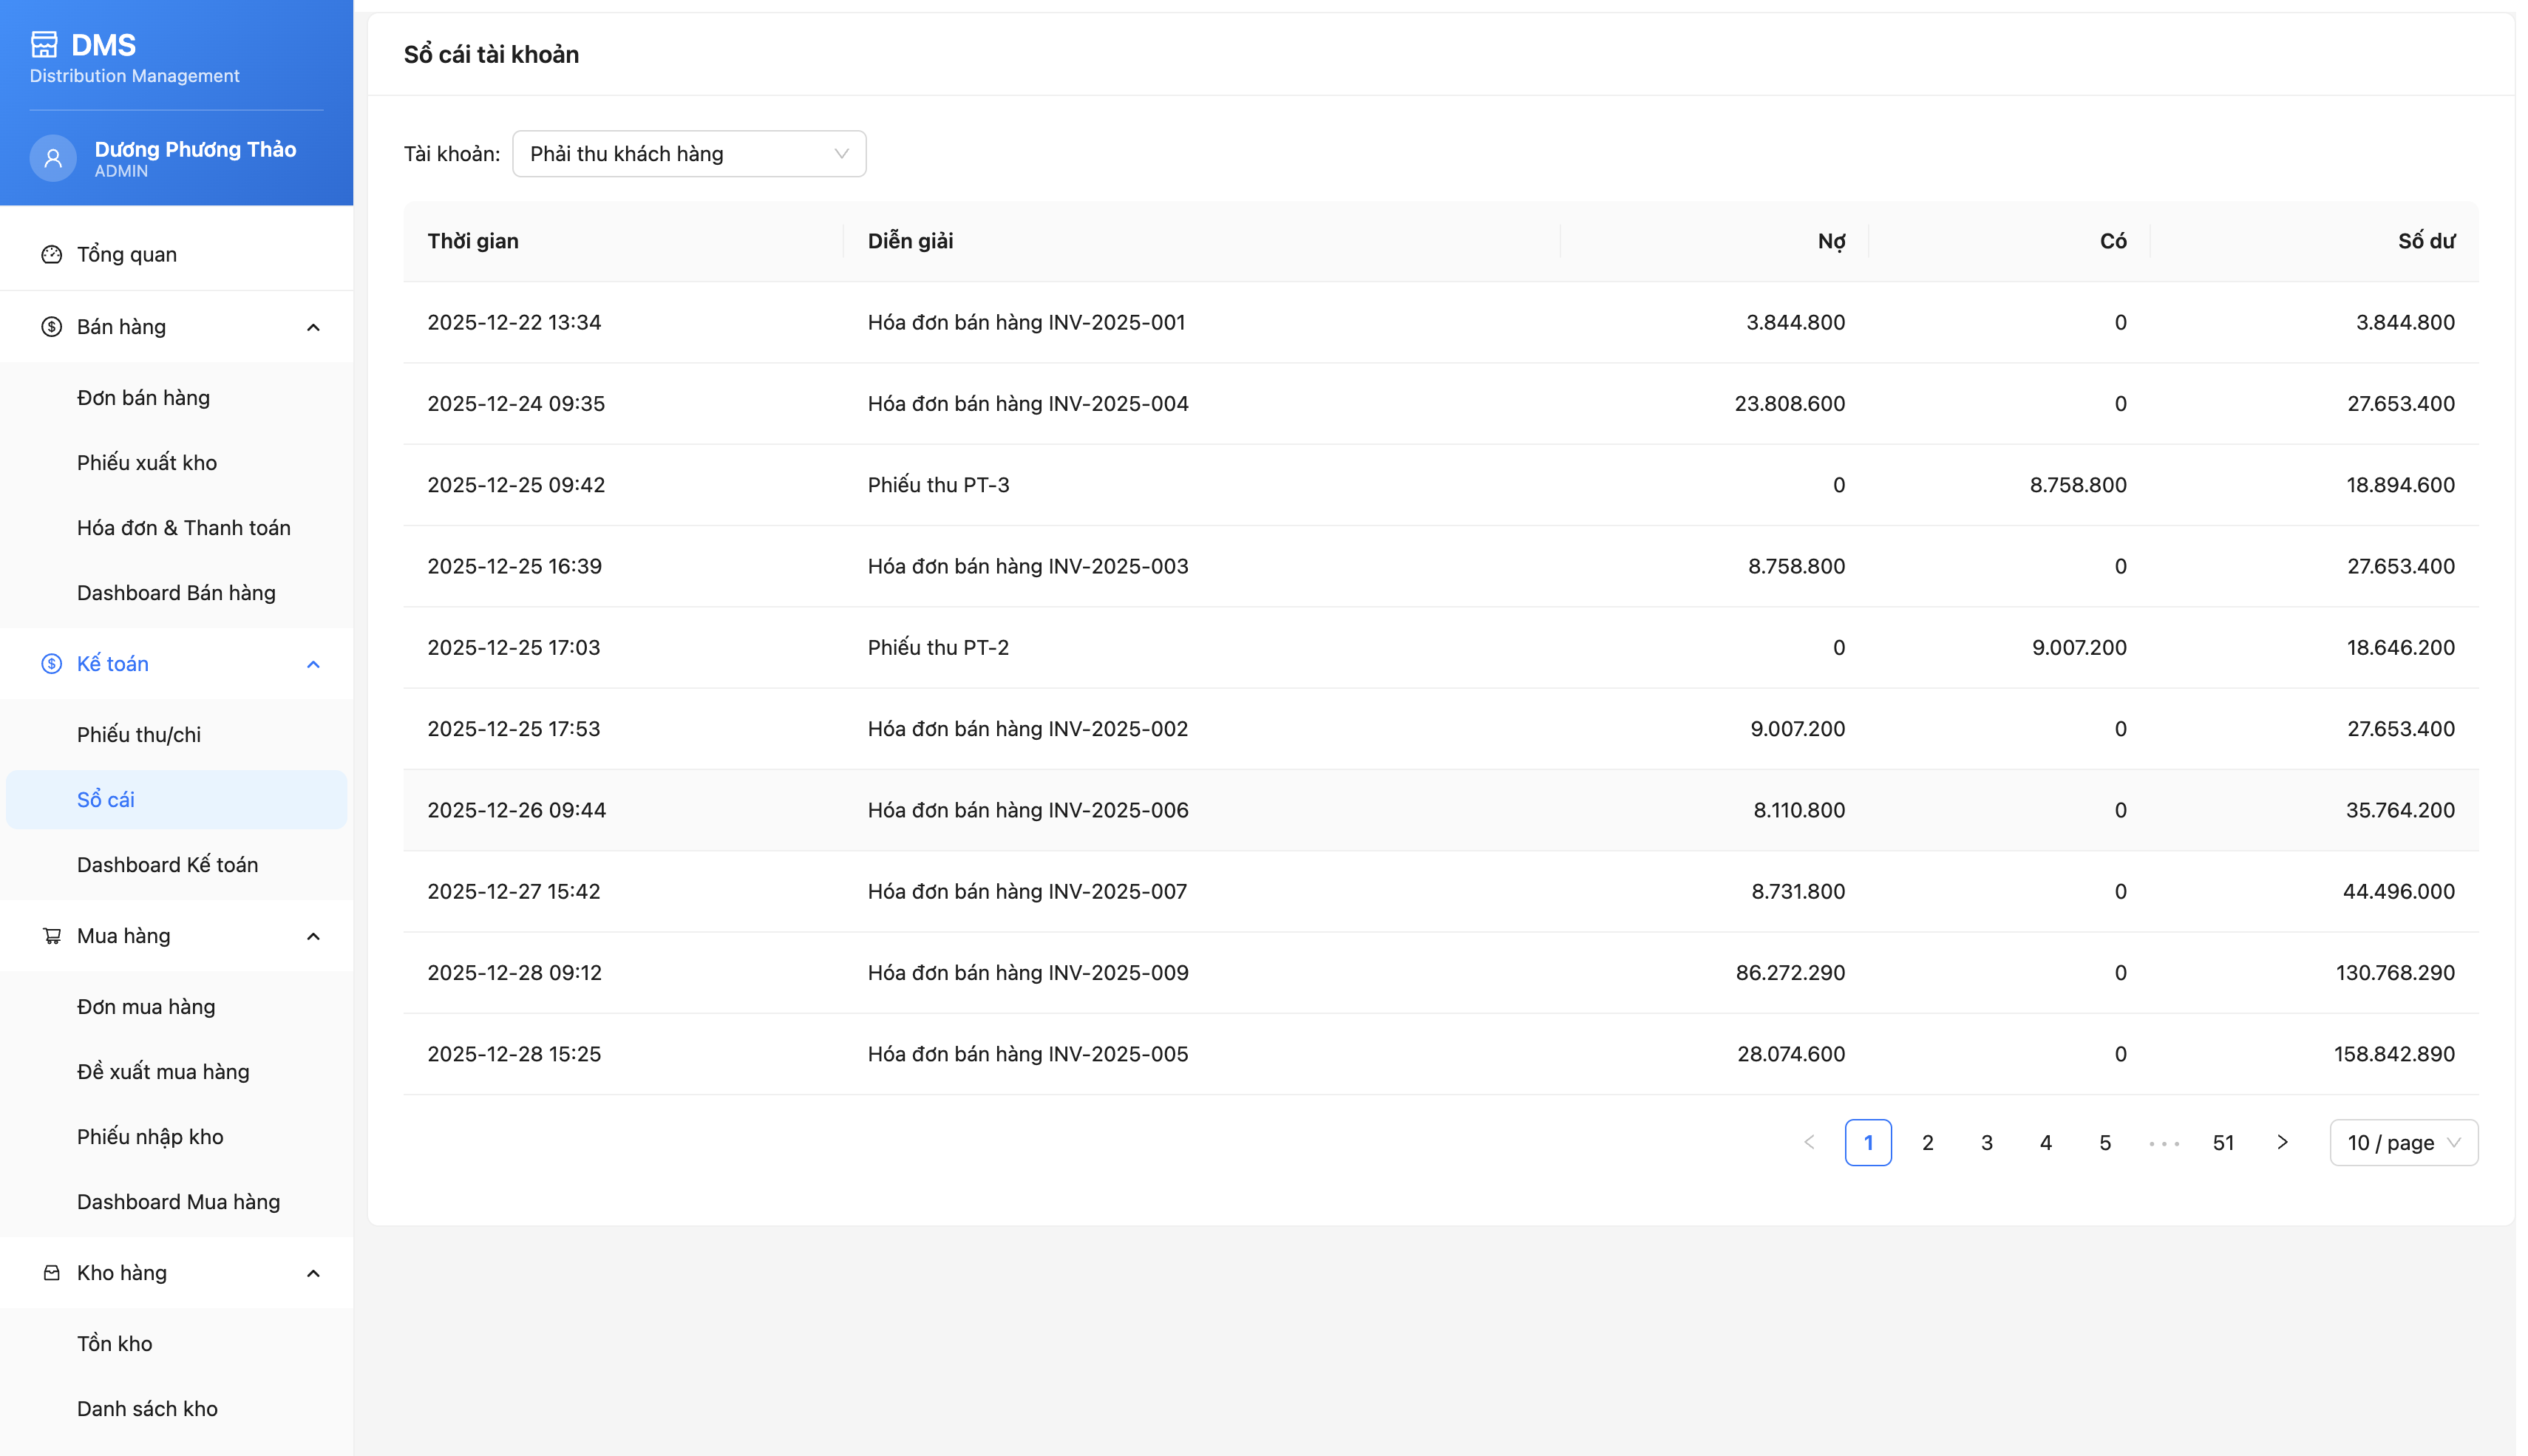
\includegraphics[width=0.95\linewidth]{Figure/screenshots/10-payment-ledger.png}
\caption{Accounts-receivable ledger with running balance}\label{fig:ui-ledger}
\end{figure}

Figure~\ref{fig:ui-ledger} shows the ledger of the accounts-receivable account.
Every sales invoice posts a debit entry and every payment receipt posts a credit
entry, and the running-balance column on the right is recomputed after each
posting. Because the same posting that debits this account credits the
corresponding revenue or cash account, the ledger is the user-facing evidence of
the double-entry accounting model described in Chapter~\ref{chapter:Contribution}.

Taken together, these screenshots confirm that the implemented system realises the
full inbound-to-settlement workflow on real data. The next section reports how the
business rules underlying these functions are verified by automated and manual
tests.

\section{Testing}
The system was verified with two complementary techniques: automated tests that
pin down the business rules with the highest consistency risk, and manual
end-to-end scenario tests that exercise the full workflow through the user
interface.

\subsection{Automated tests}
The automated suite contains thirteen tests grouped into seven classes. It runs
on an in-memory H2 database under the \texttt{test} Spring profile, so it is
self-contained and repeatable without an external database. Table~\ref{tab:autotests}
summarises the suite; all thirteen tests pass. The tests deliberately target the
points where correctness is hardest to guarantee: first-expired-first-out (FEFO)
lot allocation, stock reservation, concurrent stock deduction, double-entry
ledger balances, the credit-limit rule, and endpoint authorisation.

\begin{table}[H]\centering
\caption{Automated test suite (all passing)}
\label{tab:autotests}
\resizebox{\linewidth}{!}{%
\begin{tabular}{|l|c|l|}
\hline
\textbf{Test class} & \textbf{Tests} & \textbf{Verifies} \\ \hline
FefoAllocationTest & 2 & FEFO query order; earliest-expiry lot consumed first \\ \hline
ReservationTest & 3 & reserve raises reserved and lowers available; over-reserve rejected \\ \hline
ConcurrencyLotTest & 1 & two concurrent issues serialised; no lost update at lot level \\ \hline
AccountingServiceTest & 2 & running ledger balance; zero-amount postings skipped \\ \hline
CreditLimitRuleTest & 3 & credit-limit rule evaluated at the boundary \\ \hline
RbacSecurityTest & 1 & protected endpoint without a token is rejected \\ \hline
CoreFlowTest & 1 & application context loads with all beans wired \\ \hline
\end{tabular}%
}
\end{table}

\subsection{Critical-function test cases}
Table~\ref{tab:tests} lists the three most important functional cases together
with their observed results. TC01 is the most important case because it checks
both the aggregate inventory and the lot-level FEFO deduction: with two lots of
different expiry dates, the earliest-expiry lot is fully consumed before any
quantity is taken from the later lot. TC02 checks that reserving stock raises the
reserved quantity and lowers the available quantity while the on-hand quantity is
unchanged, which prevents overselling before goods leave the warehouse. TC03
checks the credit-limit rule, which rejects a purchase when the resulting balance
would exceed the customer credit limit.

\begin{table}[H]\centering
\caption{Critical-function test cases and results}
\label{tab:tests}
\resizebox{\linewidth}{!}{%
\begin{tabular}{|c|l|l|l|c|}
\hline
\textbf{ID} & \textbf{Function} & \textbf{Input} & \textbf{Expected} & \textbf{Result} \\ \hline
TC01 & Confirm GI (FEFO) & two lots, near/far expiry & earliest-expiry lot consumed first & Pass \\ \hline
TC02 & Approve SO (reserve) & qty $\leq$ available & reserved up, available down, on-hand same & Pass \\ \hline
TC03 & Credit-limit rule & balance+amt $>$ limit & purchase rejected by the rule & Pass \\ \hline
\end{tabular}%
}
\end{table}

The three cases are backed by \texttt{FefoAllocationTest}, \texttt{ReservationTest},
and \texttt{CreditLimitRuleTest} respectively, so they are reproducible rather than
one-off manual checks. One limitation is recorded for transparency: the
credit-limit rule is implemented and tested as a domain method, but it is not yet
invoked in the sales-order approval path, which currently enforces only stock
availability; connecting the rule to order approval is left as future work. In
addition to the automated suite, the full business workflow PO $\to$ GR $\to$ SO
approval $\to$ GI $\to$ delivery $\to$ invoice $\to$ payment was exercised
manually through the web interface against a seeded database, and the resulting
screens are presented earlier in this chapter as the illustration of the main
functions.

\section{Deployment}
\label{sec:deployment}
% GUIDE: deployment model, server/equipment specs, configuration, and any test
% deployment results (users, response time, load).
\thesisfig{deployment}{Deployment diagram}{fig:deploy}
The deployment model in Figure~\ref{fig:deploy} contains three runtime
components. The React frontend is served by the Vite development server during
development at port 5173, or by a static web server in a production-like
deployment. The Spring Boot backend runs as a Java application at port 8080 and
exposes REST APIs under \texttt{/api}. PostgreSQL runs as the database server,
using the default port 5432 in the local development environment.

For local demonstration, the backend is started with \texttt{mvn
spring-boot:run} and the frontend is started with \texttt{npm run dev}. The
frontend communicates with the backend through Axios. Authentication requests
return JWT tokens, and subsequent API calls include the token for authorization.
The backend connects to PostgreSQL using the configuration in
\texttt{application.yml}. In a production deployment, the same logical structure
can be placed behind a reverse proxy, with HTTPS termination at the proxy and
environment variables used for database credentials and JWT secrets.
